%% =====================================================================
%% Soccer match outcome prediction — Big Data Journal manuscript draft
%% Built on Springer Nature sn-jnl template (sn-mathphys-num style).
%%
%% Replace this preamble with the exact one from the journal template
%% your professor uses (sn-article.tex). The body below is plug-and-play.
%% =====================================================================

\documentclass[pdflatex,sn-mathphys-num]{sn-jnl}

\usepackage{graphicx}
\usepackage{multirow}
\usepackage{amsmath,amssymb,amsfonts}
\usepackage{amsthm}
\usepackage{mathrsfs}
\usepackage[title]{appendix}
\usepackage{xcolor}
\usepackage{textcomp}
\usepackage{manyfoot}
\usepackage{booktabs}
\usepackage{algorithm}
\usepackage{algorithmicx}
\usepackage{algpseudocode}
\usepackage{listings}
\usepackage{url}
\usepackage{tikz}
\usepackage{booktabs}  % 用于专业的三线表格式

\theoremstyle{thmstyleone}
\newtheorem{theorem}{Theorem}
\newtheorem{proposition}[theorem]{Proposition}
\theoremstyle{thmstyletwo}
\newtheorem{example}{Example}
\newtheorem{remark}{Remark}
\theoremstyle{thmstylethree}
\newtheorem{definition}{Definition}

\raggedbottom

\begin{document}

%% =====================================================================
%% TITLE / AUTHORS
%% =====================================================================

\title[Data-driven prediction of Soccer Outcome]{%
Data-driven prediction of Soccer Outcome:\\
Quantifying the Information Value of Pre-match, Half-Time and Momentum Signals across the Top-Five European Leagues}

\author*[1]{\fnm{Zhang} \sur{Gaoyuan}}\email{zhangga@kean.edu}
\author[1]{\fnm{Second} \sur{Author}}\email{second.author@example.edu}
\author[1]{\fnm{Third} \sur{Author}}\email{third.author@example.edu}

\affil*[1]{\orgdiv{Department of Computer Science},
  \orgname{Wenzhou-Kean University},
  \orgaddress{\city{Wenzhou}, \country{China}}}

%% =====================================================================
%% ABSTRACT
%% =====================================================================

\abstract{%
Predicting the outcome of association-football matches (home win, draw, away
win) is a well-studied but persistently difficult three-class problem,
dominated by intrinsic match noise, severe imbalance against draws, and
temporal drift across seasons. We present a reproducible, end-to-end
pipeline that benchmarks seven classical, deep-learning, and sequence
classifiers, plus two ensembles, on roughly $1.8\times10^{4}$ matches
drawn from ten seasons (2015/16--2024/25) of the top-five European
leagues (Premier League,
La~Liga, Serie~A, Bundesliga, Ligue~1). The pipeline integrates a multi-stage
feature-engineering chain that yields three families of inputs---pre-match
performance proxies (PPG, expected goals), market-implied probabilities,
and form/momentum/rest/head-to-head signals---together with optional
half-time observables (HT score, HT lead, HT cards). A strict
season-based time-series split prevents look-ahead leakage. We make three
contributions: (i) a controlled \emph{pre-match versus half-time}
comparison under a fixed model space, isolating the marginal information
value of forty-five minutes of play; (ii) a draw-aware evaluation
protocol combining accuracy, log-loss, F1-macro, per-class
precision/recall, and one-vs-rest ROC-AUC; and (iii) an ablation that
quantifies the predictive contribution of each feature family. Across all
leagues, gradient boosting (XGBoost) is the strongest single learner;
half-time observation adds \emph{TBD~percentage points} of accuracy and
roughly halves log-loss; class-weight scheduling and threshold tuning
lift draw recall \emph{TBD~pp} with negligible loss to home/away
precision. The pipeline and trained models are released as open source.}

\keywords{soccer prediction, machine learning, ensemble learning,
class imbalance, time-series cross-validation, expected goals,
betting odds, big data}

\maketitle

%% =====================================================================
%% 1. INTRODUCTION
%% =====================================================================
\section{Introduction}\label{sec:intro}

Association football is the most-watched sport in the world, and the
outcome of an individual match---home win, draw, or away win, denoted
\textsc{H/D/A}---has direct economic consequences for betting markets,
clubs, broadcasters and fantasy-sport operators. The forecasting problem
is, however, notoriously hard: matches are short, low-scoring, and noisy;
information is unevenly distributed between bookmakers and the public;
and the three classes are systematically imbalanced against draws.
A decade of research has converged on a typical accuracy of
$0.50$--$0.55$ for league-level pre-match prediction in Europe, with
draw recall often below $0.30$~\cite{bib1,bib2}.

Three weaknesses persist in the published record. First, most studies
\emph{stop at pre-match prediction} and ignore in-game updating, even
though the marginal value of half-time information is the central
question for live-betting and tactical analytics. Second, evaluation
typically reports only accuracy or weighted F1, masking the under-modelled
draw class. Third, several widely-cited results use random or
\emph{k}-fold cross-validation, which leaks future seasons into training
folds and inflates test scores under realistic deployment.

This paper closes those gaps with a single, reproducible pipeline. We
treat the problem as \emph{two predictions of the same target}: a
\emph{pre-match} prediction conditioned only on information known at
kickoff and a \emph{half-time} prediction that additionally observes the
half-time score, lead and cards. The model space, feature pipeline,
season-based split, and evaluation protocol are held identical, so any
delta between the two stages is attributable to the half-time signal
itself. We benchmark seven base learners (Logistic Regression, Gaussian
Naive Bayes, calibrated linear SVM, Random Forest, XGBoost,
feed-forward neural network, and Vanilla RNN) and two meta-learners (soft Voting and
Stacking), with class-weight scheduling and per-class threshold
optimisation tuned for the under-represented draw class.

Our specific contributions are:
\begin{enumerate}
  \item An open, end-to-end pipeline covering data merging, leakage-safe
        cleaning, multi-stage feature engineering, season-aware
        splitting, model training, and reporting (Section~\ref{sec:method}).
  \item A controlled pre-match versus half-time comparison over
        $\sim$18,000 matches and the top-five European leagues
        (Sections~\ref{sec:data}, \ref{sec:results}).
  \item A \emph{draw-aware evaluation protocol}: log-loss, F1-macro,
        per-class precision/recall, and OvR ROC-AUC, complementing accuracy
        (Section~\ref{sec:setup}).
  \item Feature-family ablations that quantify the marginal contribution
        of market odds, on-pitch performance proxies (PPG, xG), form/
        momentum, head-to-head, rest, and---at half-time---HT score and lead
        (Section~\ref{sec:results}).
\end{enumerate}

The remainder of the paper is organised as follows.
Section~\ref{sec:related} reviews prior work.
Section~\ref{sec:data} describes the dataset and split.
Section~\ref{sec:method} describes feature engineering, problem formulation,
model training, and tuning.
Section~\ref{sec:setup} fixes the experimental protocol.
Section~\ref{sec:results} reports results and ablations.
Section~\ref{sec:discussion} interprets the findings, and
Section~\ref{sec:conclusion} concludes.

%% =====================================================================
%% 2. RELATED WORK
%% =====================================================================
\section{Related work}\label{sec:related}

\paragraph{Statistical models.} Early pre-match prediction relied on
parametric goal-scoring processes---Poisson and bivariate-Poisson
regressions~\cite{bib3,bib4}---and on rating systems such as Elo and
TrueSkill. These models are interpretable and well-calibrated for
goal counts but struggle with the discrete \textsc{H/D/A} target,
particularly with draws.

\paragraph{Classical machine learning.} Logistic regression, Random
Forests and SVMs have been applied across leagues with reported
pre-match accuracies in the $0.50$--$0.55$ band~\cite{bib2,bib5,bib6}.
Most studies treat odds as a powerful single feature and report
that adding non-odds features yields only marginal gains.

\paragraph{Gradient boosting and ensembles.} XGBoost, LightGBM, and
soft-voting/stacking ensembles have become the dominant published
configuration in recent work~\cite{bib7,bib8}. Reported accuracies sit
in the $0.53$--$0.58$ band, with consistently weaker draw recall.

\paragraph{Neural and sequence models.} Feed-forward networks generally
match Random Forests but rarely surpass tuned XGBoost. Recurrent
networks (LSTM, GRU) have been used for in-play prediction over
event-stream data~\cite{bib9} and outperform tabular models when
high-frequency events are available, but require richer data than
match-level statistics.

\paragraph{In-play and half-time prediction.} A smaller literature
predicts the result mid-game~\cite{bib10}. The closest comparator to our
work is the reference paper of \cite{bib11}, which evaluates pre-match
classifiers on a single league. Our paper extends that line by (i)
covering five leagues and ten seasons, (ii) holding the pipeline
identical between pre-match and half-time, and (iii) reporting
draw-aware metrics with bootstrap confidence intervals.

\paragraph{Positioning.} Compared to the surveyed work we contribute a
\emph{controlled comparison} rather than a single new model, and a
\emph{deployable pipeline} with explicit leakage controls and an
imbalance-aware evaluation protocol.

%% =====================================================================
%% 3. DATA
%% =====================================================================
\section{Data}\label{sec:data}

\subsection{Data acquisition}

The primary dataset was obtained from FootyStats\footnote{\url{https://footystats.org}}, comprising match results, statistics, and betting odds for the top-five European leagues. Supplementary opening and closing odds were sourced from football-data.co.uk\footnote{\url{https://www.football-data.co.uk}} to capture market dynamics. The combined dataset spans ten seasons (2015/16--2024/25) with 18,012 matches in total.

The dataset covers the top-five European football leagues over ten complete seasons from 2015/16 to 2024/25. The ongoing 2025/26 season was deliberately excluded to ensure data completeness and avoid potential biases from unfinished fixtures. Table~\ref{tab:dataset} presents the distribution of matches across leagues.


\begin{table}[htbp]
\centering
\caption{Distribution of matches by league across seasons 2015/16--2024/25.}
\label{tab:dataset}
\begin{tabular}{@{}llr@{}}
\toprule
\textbf{League} & \textbf{Country} & \textbf{Matches} \\
\midrule
Premier League  & England & 3,800 \\
La Liga         & Spain   & 3,800 \\
Serie A         & Italy   & 3,801 \\
Ligue 1         & France  & 3,551 \\
Bundesliga      & Germany & 3,060 \\
\midrule
\textbf{Total}  &         & \textbf{18,012} \\
\bottomrule
\end{tabular}
\end{table}
\vspace{-8pt}
{\footnotesize\textit{Note:} Bundesliga (18 teams) has 306 matches per season; other leagues have 20 teams with 380 matches. Ligue 1 variations stem from league restructuring and the curtailed 2019/20 season.}

To investigate the impact of real-time momentum on match prediction, this study utilizes the open-access event-level football data provided by StatsBomb~\cite{statsbomb2023}. The StatsBomb open data initiative offers one of the most granular publicly available football datasets, containing detailed sequential records of on-ball actions for each match.

Due to the availability constraints of the free data tier, our analysis focuses exclusively on the 2015/16 season across Europe's top five leagues, since they are the only open data. Table~\ref{tab:data_coverage} summarizes the data coverage.

\begin{table}[htbp]
\centering
\caption{Data Coverage}
\label{tab:data_coverage}
\begin{tabular}{lccc}
\toprule
\textbf{League} & \textbf{Competition ID} & \textbf{Season ID} & \textbf{Matches} \\
\midrule
Premier League (England) & 2 & 27 & 380 \\
La Liga (Spain) & 11 & 27 & 380 \\
Serie A (Italy) & 12 & 27 & 380 \\
Bundesliga (Germany) & 9 & 27 & 306 \\
Ligue 1 (France) & 7 & 27 & 380 \\
\midrule
\textbf{Total} & -- & -- & \textbf{1,826} \\
\bottomrule
\end{tabular}
\end{table}

The data acquisition process was implemented in two stages using the official StatsBomb Python API (\texttt{statsbombpy})~\cite{statsbombpy2023}. In the first stage, we retrieved match-level metadata for each of the five target competitions, including match identifiers, dates, and team names. In the second stage, we fetched the detailed event-level data for each match based on the retrieved match identifiers. Each match's event data contains comprehensive temporal logs of all on-ball actions, including passes, shots, fouls, and other game events, along with contextual information such as timestamps, pitch coordinates, and outcome classifications.

All acquired data was stored in Apache Parquet format for efficient storage and subsequent processing. The resulting dataset comprises 1,826 matches with approximately 3 million event records, providing the foundation for constructing real-time momentum features in the following experiments.

\subsection{Train/validation/test split}\label{subsec:split}

To match deployment conditions and avoid look-ahead leakage we use a
\emph{season-based time-series split} (Table~\ref{tab:split}). All matches
of a season are assigned to a single subset.

\begin{table}[h]
\caption{Season-based time-series split.}\label{tab:split}
\begin{tabular}{@{}llr@{}}
\toprule
Subset      & Seasons                            & \# matches \\
\midrule
Training    & 2015/16, 2016/17, 2017/18, 2018/19, 2019/20, 2020/21 & 11,928 \\
Validation  & 2021/22, 2022/23                   & 3,800 \\
Test        & 2023/24, 2024/25                          & 2,284 \\
\botrule
\end{tabular}
\end{table}

\subsection{Data Cleaning and Leakage Control}
\label{subsec:leakage}

We retained only complete matches and recorded the number of missing entries. Approximately 60\% of the available features were preserved while maximising feature retention.

A central design decision is the explicit removal of post-event information to prevent data leakage. The cleaning stage removes twenty-six full-match and second-half columns (e.g., final shots, final xG, second-half cards) before any feature is computed. Half-time columns are retained but \emph{gated by task}: the pre-match feature builder excludes them, while the half-time feature builder includes them. Identifier and target columns are excluded from both.

Table~\ref{tab:leakage_columns} lists all leakage-prone columns removed during the cleaning stage, grouped by category.

\begin{table}[htbp]
\centering
\caption{Leakage-prone columns removed during data cleaning}
\label{tab:leakage_columns}
\begin{tabular}{@{}p{3.5cm}p{9.5cm}@{}}
\toprule
\textbf{Category} & \textbf{Columns} \\
\midrule
Full-time results & \texttt{home\_team\_goal\_count}, \texttt{away\_team\_goal\_count}, \texttt{total\_goal\_count}, \texttt{full\_time\_result}, \texttt{ft\_result}, \texttt{result} \\
\midrule
Full-time statistics & \texttt{home\_team\_possession}, \texttt{away\_team\_possession}, \texttt{home\_team\_shots}, \texttt{away\_team\_shots}, \texttt{home\_team\_shots\_on\_target}, \texttt{away\_team\_shots\_on\_target}, \texttt{home\_team\_shots\_off\_target}, \texttt{away\_team\_shots\_off\_target}, \texttt{home\_team\_corners}, \texttt{away\_team\_corners}, \texttt{home\_team\_corner\_count}, \texttt{away\_team\_corner\_count}, \texttt{home\_team\_fouls}, \texttt{away\_team\_fouls} \\
\midrule
Full-time cards & \texttt{home\_team\_yellow\_cards}, \texttt{away\_team\_yellow\_cards}, \texttt{home\_team\_red\_cards}, \texttt{away\_team\_red\_cards}, \texttt{home\_team\_cards}, \texttt{away\_team\_cards} \\
\midrule
Second-half statistics & \texttt{home\_team\_goal\_count\_second\_half}, \texttt{away\_team\_goal\_count\_second\_half}, \texttt{total\_goals\_second\_half}, \texttt{home\_team\_second\_half\_cards}, \texttt{away\_team\_second\_half\_cards}, \texttt{home\_team\_yellow\_cards\_second\_half}, \texttt{away\_team\_yellow\_cards\_second\_half}, \texttt{home\_team\_red\_cards\_second\_half}, \texttt{away\_team\_red\_cards\_second\_half}, \texttt{home\_team\_shots\_second\_half}, \texttt{away\_team\_shots\_second\_half}, \texttt{home\_team\_shots\_on\_target\_second\_half}, \texttt{away\_team\_shots\_on\_target\_second\_half}, \texttt{home\_team\_corners\_second\_half}, \texttt{away\_team\_corners\_second\_half}, \texttt{home\_team\_fouls\_second\_half}, \texttt{away\_team\_fouls\_second\_half} \\
\midrule
Average ppg across season  & \texttt{home\_ppg}, \texttt{away\_ppg} \\
\midrule
Expected goals & \texttt{team\_a\_xg}, \texttt{team\_b\_xg} \\
\midrule
Goal timings & \texttt{home\_team\_goal\_timings}, \texttt{away\_team\_goal\_timings} \\
\botrule
\end{tabular}
\end{table}

By removing these columns before any feature computation, we ensure that no post-match information contaminates the pre-match or half-time prediction tasks.

%% =====================================================================
%% 4. METHODOLOGY
%% =====================================================================
\section{Methodology}\label{sec:method}

This section describes the modelling methodology, including feature engineering, problem formulation, model training, imbalance handling, and hyper-parameter tuning.

\subsection{Feature engineering}\label{sec:features}

This subsection describes the construction of predictive features used in the pre-match and half-time prediction tasks. The feature-engineering pipeline is organised into two parts. Section~\ref{subsec:match-level-feature-engineering} describes match-level feature engineering based on historical match records, odds, team form, rest, congestion, and travel information. Section~\ref{subsec:real-time-momentum-feature-engineering} details real-time momentum feature engineering based on event-level data; these momentum features are merged into the match-level table for 2015/16 season matches across all five leagues.

\subsubsection{Match-level feature engineering}
\label{subsec:match-level-feature-engineering}

We construct match-level features in five successive stages, each implemented
as a self-contained script. Stage outputs are persisted to enable
reproducibility and inspection.

\paragraph{Stage 1 --- Table Assembly}\label{subsec:stage1-table-assembly}

This stage assembles the raw match-level dataset from FootyStats, comprising 67 fields from the original data source. The dataset encompasses match fixtures, pre-match team metrics, betting market data, and half-time statistics. Leakage-prone features are excluded before any derived features are computed. Table~\ref{tab:stage1_features} summarises the feature categories and their availability for each prediction task.

\begin{table}[htbp]
\centering
\caption{Feature categories from the assembled match table.}
\label{tab:stage1_features}
\begin{tabular}{@{}p{3.2cm}p{5.8cm}cc@{}}
\toprule
\textbf{Category} & \textbf{Description} & \textbf{Pre-match} & \textbf{Half-time} \\
\midrule
\multicolumn{4}{l}{\textit{Original Data Features}} \\
\midrule
Match Information & Season, date, home/away teams, venue, referee, game week & \checkmark & \checkmark \\
Pre-match PPG & Pre-Match PPG (Home/Away) --- average points per game before match & \checkmark & \checkmark \\
Pre-match xG & Home/Away Team Pre-Match xG, team\_a/b\_xG --- expected goals & \checkmark & \checkmark \\
Pre-match Predictions & Average goals, BTTS \%, over/under thresholds (1.5--4.5 goals) & \checkmark & \checkmark \\
Betting Odds & Full-time odds (home/draw/away), over/under odds, BTTS odds & \checkmark & \checkmark \\
Half-time Statistics & Goals at half-time, first-half cards & -- & \checkmark \\
\midrule
\multicolumn{4}{l}{\textit{Derived Features}} \\
\midrule
ppg\_differential & Home PPG $-$ Away PPG (relative strength indicator) & \checkmark & \checkmark \\
xg\_power\_index & Home xG $-$ Away xG (attacking strength indicator) & \checkmark & \checkmark \\
ht\_result & Half-time result encoded as H/D/A & -- & \checkmark \\
half\_time\_lead & Home team goal lead at half-time (signed integer) & -- & \checkmark \\
\bottomrule
\end{tabular}
\end{table}
\vspace{-8pt}
{\footnotesize\textit{Note:} \checkmark~indicates feature availability for model training; ``--'' indicates unavailability. Post-match statistics (full-time goals, shots, possession, etc.) are excluded as they constitute target leakage.}

\paragraph{Stage 2 --- Odds Integration}\label{subsec:odds}

This stage enriches the betting odds data by integrating opening and closing odds from football-data.co.uk\footnote{\url{https://www.football-data.co.uk}}, a supplementary data source providing historical bookmaker odds. The original dataset contains only closing odds for match results, over/under goals, and BTTS markets. This stage adds opening odds and computes derived features that capture market dynamics.

Opening and closing odds are sourced with the following priority: Bet365, Pinnacle, Market Average, and Market Maximum. For each match, the odds for the 1X2 market (home win, draw, away win) are extracted and the following features are derived:

\begin{equation}
\text{Implied Probability: } p_{i} = \frac{1}{o_{i}}, \quad i \in \{\text{home, draw, away}\}
\label{eq:implied}
\end{equation}

\begin{equation}
\text{Odds Movement: } \Delta o_{i} = o^{close}_{i} - o^{open}_{i}
\label{eq:odds_move}
\end{equation}

\begin{equation}
\text{Probability Shift: } \Delta p_{i} = p^{close}_{i} - p^{open}_{i}
\label{eq:prob_shift}
\end{equation}

\begin{equation}
\text{Overround: } \Omega = \sum_{i} p_{i} = \sum_{i} \frac{1}{o_{i}}
\label{eq:overround}
\end{equation}

where $o_{i}$ denotes the decimal odds for outcome $i$. The overround $\Omega$ quantifies the bookmaker's margin, with values greater than 1 indicating the implied bookmaker edge.

Table~\ref{tab:odds_features} lists all odds-related features derived in this stage.

\begin{table}[htbp]
\centering
\caption{Odds integration features derived in Stage 2.}
\label{tab:odds_features}
\begin{tabular}{@{}p{3.5cm}p{5.5cm}cc@{}}
\toprule
\textbf{Category} & \textbf{Features} & \textbf{Pre-match} & \textbf{Half-time} \\
\midrule
Opening odds & \texttt{odds\_open\_home}, \texttt{odds\_open\_draw}, \texttt{odds\_open\_away} & \checkmark & \checkmark \\
Closing odds & \texttt{odds\_close\_home}, \texttt{odds\_close\_draw}, \texttt{odds\_close\_away} & \checkmark & \checkmark \\
Odds source & \texttt{odds\_open\_source}, \texttt{odds\_close\_source} & \checkmark & \checkmark \\
\midrule
Odds movement & \texttt{odds\_move\_home}, \texttt{odds\_move\_draw}, \texttt{odds\_move\_away} & \checkmark & \checkmark \\
Absolute movement & \texttt{odds\_move\_abs\_home}, \texttt{odds\_move\_abs\_draw}, \texttt{odds\_move\_abs\_away} & \checkmark & \checkmark \\
\midrule
Implied prob.\ (open) & \texttt{implied\_prob\_open\_home}, \texttt{implied\_prob\_open\_draw}, \texttt{implied\_prob\_open\_away} & \checkmark & \checkmark \\
Implied prob.\ (close) & \texttt{implied\_prob\_close\_home}, \texttt{implied\_prob\_close\_draw}, \texttt{implied\_prob\_close\_away} & \checkmark & \checkmark \\
Probability shift & \texttt{implied\_prob\_shift\_home}, \texttt{implied\_prob\_shift\_draw}, \texttt{implied\_prob\_shift\_away} & \checkmark & \checkmark \\
\midrule
Overround & \texttt{overround\_open}, \texttt{overround\_close} & \checkmark & \checkmark \\
\bottomrule
\end{tabular}
\end{table}

These features capture both the initial market consensus (opening odds) and late market adjustments (closing odds and movements). The odds movement features proxy late information incorporation, such as team news or market sentiment shifts, while the overround indicates bookmaker pricing efficiency.

Note that the closing odds from Stage 1 (\texttt{odds\_ft\_*}) and Stage 2 (\texttt{odds\_close\_*}) originate from different data sources and serve complementary purposes: Stage 1 provides broader market coverage including over/under and BTTS, while Stage 2 enables temporal analysis through opening-closing comparisons.

\paragraph{Stage 3 --- Historical Performance and Team Strength}\label{subsec:historical}

This stage computes long-term team characteristics using only matches played prior to the current fixture, ensuring no look-ahead bias. The features are organised into two categories: (1) historical performance metrics, including cumulative win/draw/loss rates, goals for/against, goal differentials, win/loss margins, head-to-head records, and current streaks; and (2) team strength indicators, including league standings and Elo ratings. All features are available for both pre-match and half-time prediction tasks.

The Elo rating system provides a dynamic measure of team strength, updated after each match according to:

\begin{equation}
E_{\text{home}} = \frac{1}{1 + 10^{-(R_{\text{home}} + \alpha - R_{\text{away}})/400}}
\label{eq:elo_expected}
\end{equation}

\begin{equation}
R'_{\text{home}} = R_{\text{home}} + K \cdot (S_{\text{home}} - E_{\text{home}}), \quad R'_{\text{away}} = R_{\text{away}} - K \cdot (S_{\text{home}} - E_{\text{home}})
\label{eq:elo_update}
\end{equation}

where $R_{\text{home}}$ and $R_{\text{away}}$ are the pre-match Elo ratings, $\alpha = 60$ is the home advantage adjustment, $K = 20$ is the update factor, $S_{\text{home}} \in \{1, 0.5, 0\}$ is the actual match outcome from the home team's perspective (win, draw, loss), and $E_{\text{home}}$ is the expected score. Each team starts with an initial rating of 1500, and ratings are maintained separately for each league.

Table~\ref{tab:historical_features} lists all features derived in this stage, grouped by category.

\begin{table}[htbp]
\centering
\caption{Historical performance, head-to-head, streak, ranking, and rating features.}
\label{tab:historical_features}
\begin{tabular}{@{}p{3.5cm}p{5.5cm}cc@{}}
\toprule
\textbf{Category} & \textbf{Features} & \textbf{Pre-match} & \textbf{Half-time} \\
\midrule
Win/draw/loss rates & \texttt{Total home/away win/draw/loss rate} (6 features) & \checkmark & \checkmark \\
Cumulative goals & \texttt{Home/away goals forward/against/diff} (6 features) & \checkmark & \checkmark \\
Per-match averages & \texttt{Home/away goals per match} (6 features) & \checkmark & \checkmark \\
Margin of victory/defeat & \texttt{Home/away wins/losses margin goal} (4 features) & \checkmark & \checkmark \\
\midrule
Head-to-head (all time) & \texttt{h2h\_matches\_played}, \texttt{h2h\_home\_wins}, \texttt{h2h\_draws}, \texttt{h2h\_away\_wins}, \texttt{h2h\_home\_win\_rate} & \checkmark & \checkmark \\
Head-to-head (recent 10) & \texttt{h2h\_recent\_home/draw/away\_wins} (3 features) & \checkmark & \checkmark \\
\midrule
Current streaks & \texttt{home/away current/unbeaten/winless streak} (6 features) & \checkmark & \checkmark \\
League standings & \texttt{home/away current rank}, \texttt{rank\_difference}, \texttt{home/away points before match}, \texttt{points\_difference} & \checkmark & \checkmark \\
\midrule
Elo ratings & \texttt{home\_elo\_pre}, \texttt{away\_elo\_pre}, \texttt{elo\_diff\_pre} & \checkmark & \checkmark \\
\bottomrule
\end{tabular}
\end{table}

The head-to-head record includes both all-time encounters and a restricted window of the most recent ten matches. Streak features track current momentum: positive values indicate winning streaks, negative values indicate losing streaks, while unbeaten and winless streaks capture longer-term resilience or struggles. League standings and points differences provide context on each team's seasonal performance level. The Elo rating captures long-term team strength evolution across seasons.


\paragraph{Stage 4 --- Recent Form and Momentum}\label{subsec:form}

Rolling-window features over the last $k \in \{3, 5, 8\}$ matches capture short-term dynamics, including form points, goal differential, xG momentum, volatility, and opponent-adjusted strength. Additionally, venue-specific form isolates performance when playing at home or away, and rolling odds movements proxy market momentum. Table~\ref{tab:form_features} lists all form and momentum features derived in this stage.

\begin{table}[htbp]
\centering
\caption{Form and momentum features.}
\label{tab:form_features}
\begin{tabular}{@{}p{3.5cm}p{5.5cm}cc@{}}
\toprule
\textbf{Category} & \textbf{Features} & \textbf{Pre-match} & \textbf{Half-time} \\
\midrule
Disciplinary metrics & \texttt{home/away\_recent\_cards}, \texttt{home/away\_recent\_fouls} & \checkmark & \checkmark \\
\midrule
Form points (windows 3,5,8) & \texttt{home/away\_form\_pts\_3/5/8}, \texttt{form\_pts\_diff\_3/5/8} & \checkmark & \checkmark \\
Goal/xG momentum (window 5) & \texttt{home/away\_goal\_diff\_5}, \texttt{goal\_diff\_mom\_5\_diff}, \texttt{home/away\_xg\_diff\_5\_proxy}, \texttt{xg\_diff\_mom\_5\_proxy\_diff} & \checkmark & \checkmark \\
Trend and volatility & \texttt{home/away\_mom\_slope}, \texttt{mom\_slope\_diff}, \texttt{home/away\_mom\_volatility\_5}, \texttt{mom\_volatility\_diff} & \checkmark & \checkmark \\
Venue-specific form (window 5) & \texttt{home/away\_venue\_form\_pts\_5}, \texttt{venue\_form\_pts\_5\_diff}, \texttt{home/away\_venue\_xg\_diff\_5\_proxy}, \texttt{venue\_xg\_diff\_5\_proxy\_diff} & \checkmark & \checkmark \\
Odds momentum (window 5) & \texttt{home/away\_odds\_move\_for\_ewm\_5}, \texttt{odds\_move\_for\_ewm\_diff\_5}, \texttt{home/away\_implied\_prob\_shift\_for\_ewm\_5}, \texttt{implied\_prob\_shift\_for\_ewm\_diff\_5}, \texttt{odds\_move\_abs\_for\_mom\_diff\_5} & \checkmark & \checkmark \\
Opponent-adjusted form (window 5) & \texttt{home/away\_opp\_adj\_form\_5}, \texttt{opp\_adj\_form\_diff\_5}, \texttt{home/away\_opp\_adj\_form\_5\_elo}, \texttt{opp\_adj\_form\_diff\_5\_elo} & \checkmark & \checkmark \\
\bottomrule
\end{tabular}
\end{table}

The slope features capture whether a team's form is improving or declining, while volatility measures consistency. Opponent-adjusted form uses Elo ratings to weight the strength of recent opponents, providing a more accurate assessment of true performance.

\paragraph{Stage 5 --- Rest, Congestion, and Travel}\label{subsec:rest}

Days since last match for each side, rolling match density (matches
played in the last 14/30 days), back-to-back fixtures, and proxy
fatigue scores are computed. Travel distance and accumulated fatigue
are particularly relevant for teams participating in European
competitions or facing long-distance away fixtures. The rest days feature is defined as:

\begin{equation}
\texttt{rest\_days} = \text{current\_match\_date} - \text{last\_match\_date}
\end{equation}

Match density momentum captures the rolling average of fixture congestion:

\begin{equation}
\texttt{match\_density\_mom\_5} = \frac{1}{5} \sum_{i=1}^{5} \text{match\_density}_i
\end{equation}

An exponential weighted moving average (EWM) with span 5 is also computed:

\begin{equation}
\texttt{match\_density\_ewm\_5} = \text{EWM}_{\alpha=2/(5+1)}(\text{match\_density})
\end{equation}

The away team fatigue score incorporates travel distance, fixture congestion,
and rest days:

\begin{equation}
\texttt{away\_travel\_fatigue\_score} = \log(1 + \text{travel\_km}) \times
\left(1 + \text{match\_density}\right) / \sqrt{\text{rest\_days} + 1}
\end{equation}

Travel momentum features follow the same rolling average and EWM formulations.
Table~\ref{tab:rest_features} lists all rest, congestion, and travel features
derived in this stage.

\begin{table}[htbp]
\centering
\caption{Rest, congestion, and travel features.}
\label{tab:rest_features}
\begin{tabular}{@{}p{3.5cm}p{5.5cm}cc@{}}
\toprule
\textbf{Category} & \textbf{Features} & \textbf{Pre-match} & \textbf{Half-time} \\
\midrule
Rest days & \texttt{home\_rest\_days}, \texttt{away\_rest\_days} & \checkmark & \checkmark \\
Match density & \texttt{home/away\_match\_density\_mom\_5}, \texttt{home/away\_match\_density\_ewm\_5} & \checkmark & \checkmark \\
Travel distance & \texttt{home\_travel\_km\_team}, \texttt{away\_travel\_km\_team} & \checkmark & \checkmark \\
Travel momentum (window 5) & \texttt{home/away\_travel\_km\_mom\_5}, \texttt{home/away\_travel\_km\_ewm\_5} & \checkmark & \checkmark \\
Fatigue score & \texttt{away\_travel\_fatigue\_score}, \texttt{home/away\_travel\_fatigue\_mom\_5} & \checkmark & \checkmark \\
\bottomrule
\end{tabular}
\end{table}

The home team's travel distance is set to zero by convention, as they
are playing at their home venue. Fatigue scores are designed to penalise
teams facing long travel, high fixture congestion, and limited recovery time.


\subsubsection{Real-time momentum feature engineering}\label{subsec:real-time-momentum-feature-engineering}\label{sec:momentum_features}

This section describes the construction of real-time momentum features from event-level match data. The feature engineering pipeline comprises two stages: (1) event state table construction, which transforms raw event streams into structured time-series states, and (2) momentum signal computation and curve-based feature extraction.

\paragraph{Event state table construction}\label{sec:event_state_table}

The raw event-level data obtained from StatsBomb consists of a sequential stream of on-ball actions (e.g., passes, shots, fouls) for each match. To enable momentum modeling, we transform this event stream into a structured event state table where each row represents the match state at a discrete moment in time.

\subparagraph{Temporal Alignment and Event Filtering.}
For each match, events are sorted chronologically by period, minute, and second. Administrative events that do not represent substantive match actions---specifically Starting XI, Half Start, Half End, Tactical Shift, Referee Ball-Drop, and Injury Stoppage---are excluded from the state table. Each retained event serves as a state point, capturing the match context at that specific timestamp.

\subparagraph{Rolling-Window Feature Computation.}
At each state point, we compute a set of rolling-window features that quantify recent match activity for both the home and away teams. These features are calculated over fixed temporal windows preceding each event timestamp. Table~\ref{tab:rolling_features} summarises the computed features and their respective window sizes.

\begin{table}[htbp]
\centering
\caption{Rolling-Window Feature Definitions}
\label{tab:rolling_features}
\begin{tabular}{llc}
\toprule
\textbf{Feature Category} & \textbf{Description} & \textbf{Window (sec)} \\
\midrule
Recent Shots & Count of shot events & 60 \\
Recent Expected Goals (xG) & Sum of shot xG values & 60 \\
Recent Corners & Count of corner kicks & 120 \\
Recent Box Entries & Count of entries into penalty area & 60 \\
Recent High Turnovers & Count of ball recoveries in attacking third & 60 \\
\bottomrule
\end{tabular}
\end{table}

For each feature category, we compute separate values for the home team and away team, as well as the differential (home minus away). The rolling-window calculation is implemented using a vectorised cumulative sum approach, which enables efficient $O(n)$ computation for $n$ events.

\subparagraph{Game State Variables.}
In addition to the rolling-window features, we maintain cumulative game state variables that are updated incrementally throughout each match:
\begin{itemize}
    \item \textbf{Score Difference}: The goal differential from the home team's perspective ($\text{home goals} - \text{away goals}$)
    \item \textbf{Red Card Difference}: The red card differential from the home team's perspective ($\text{home red cards} - \text{away red cards}$)
\end{itemize}

\subparagraph{Target Label Construction.}
To enable supervised learning of momentum patterns, we construct a target label for each state point indicating which team (if any) scores the next goal following the current event. The label $\mathcal{L}_t \in \{\text{home}, \text{away}, \text{none}\}$ is defined as:
\begin{itemize}
    \item \textbf{home}: The next goal is scored by the home team
    \item \textbf{away}: The next goal is scored by the away team
    \item \textbf{none}: No further goals are scored in the match
\end{itemize}

This labelling scheme operationalises momentum as the propensity for a team to score the next goal, providing a natural prediction target for momentum modelling.

The complete feature set for each state point comprises 21 variables: period, time in seconds, score difference, red card difference, and the rolling-window features (home, away, and differential values for each of the five feature categories).

\paragraph{Momentum signal computation}\label{sec:momentum_computation}

Building on the event state table, we derive two complementary,
fully interpretable momentum curves for every match: a
\emph{directional} curve $M_{eq}(t)$, which captures who is outplaying
whom at moment $t$, and an \emph{intensity} curve $M_{int}(t)$, which
captures how active the match is overall. Both curves are linear
combinations of observable event counts with weights chosen as expert
priors. The magnitudes are calibrated against an exploratory Ridge fit
on the full $\sim$6.4 M event-state rows so that the chosen values are
consistent with the data, but the final weights are fixed constants and
the pipeline requires no model training. This makes the momentum
features fully reproducible, league-agnostic, and free of any
information leakage between matches.

\subparagraph{Directional momentum.}
The directional curve is
\begin{equation}
M_{eq}(t) = w_0 + \sum_{i \in \mathcal{F}} w_i\,\Delta_i(t)
          + w_{\text{red}}\,\Delta_{\text{red}}(t)
          + w_{\text{score}}\,\tanh\!\bigl(\beta\,\Delta_{\text{score}}(t)\bigr),
\label{eq:momentum_eq}
\end{equation}
where $\mathcal{F} = \{\text{xG}, \text{shots}, \text{box entries},
\text{corners}, \text{high turnovers}\}$, $\Delta_i(t)$ is the
home$-$away differential of the rolling-window count for feature $i$ at
time $t$, and $\Delta_{\text{score}}(t)$, $\Delta_{\text{red}}(t)$ are
the cumulative goal and red-card differentials. The hyperbolic tangent
saturates the score-difference contribution: with $\beta = 0.5$, a
one-goal lead maps to $\tanh(0.5)\approx 0.46$ and a two-goal lead to
$\approx 0.76$, so a 5--0 scoreline does not produce five times the
signal of a 1--0 scoreline. Table~\ref{tab:eq_weights} lists the
calibrated weights.

\begin{table}[htbp]
\centering
\caption{Calibrated weights for the directional momentum $M_{eq}(t)$.
The signs and relative magnitudes match an exploratory Ridge fit on the
full event-state corpus.}
\label{tab:eq_weights}
\begin{tabular}{@{}lcl@{}}
\toprule
\textbf{Term} & \textbf{Weight} & \textbf{Interpretation} \\
\midrule
$w_0$ (intercept)               & $+0.07$           & home-advantage baseline \\
$w_{\text{xG}}$                 & $+0.07$           & strongest event-level signal \\
$w_{\text{shots}}$              & $+0.01$           & weak; largely absorbed by xG \\
$w_{\text{box entries}}$        & $+0.03$           & predicts goals \\
$w_{\text{corners}}$            & $+0.02$           & weak attacking signal \\
$w_{\text{high turnovers}}$     & $\phantom{+}0.00$ & no net signal once xG known \\
$w_{\text{red}}$                & $-0.23$           & a home red card sharply lowers
                                                       the next-goal probability \\
$w_{\text{score}}$              & $+0.09$           & leading teams keep scoring (saturated) \\
\bottomrule
\end{tabular}
\end{table}

By construction $M_{eq}(t) > 0$ indicates the home team is the more
likely scorer of the next goal and $M_{eq}(t) < 0$ indicates the away
team. Because $M_{eq}$ is built from differentials, however, it is
\emph{directional only}: two evenly matched 0.7-xG teams and two passive
0.05-xG teams both yield $M_{eq}\!\approx 0$, although the matches
differ greatly in character. The intensity curve below resolves this
ambiguity.

\subparagraph{Intensity-based momentum.}
The intensity curve sums event activity across both teams:
\begin{equation}
M_{int}(t) = \sum_{i \in \mathcal{F}} |w_i|\,
             \bigl[\,x_{i,\text{home}}(t) + x_{i,\text{away}}(t)\,\bigr],
\label{eq:momentum_int}
\end{equation}
where $x_{i,\text{home}}(t)$ and $x_{i,\text{away}}(t)$ are the
rolling-window counts of feature $i$ for the home and away teams at
time $t$, and the absolute values $|w_i|$ are reused from $M_{eq}$ so
that the two curves are calibrated on a common scale of importance.
Cumulative state variables ($\Delta_{\text{score}}$,
$\Delta_{\text{red}}$) are intentionally excluded from $M_{int}$: they
describe game state rather than event-rate intensity and are already
encoded in $M_{eq}$. By construction $M_{int}(t) \ge 0$, and a high
value indicates a high-tempo match regardless of which team dominates.

\subparagraph{Curve-based feature extraction for half-time prediction.}
For each match we restrict both curves to the first half
($\text{period}=1$) and resample them onto a uniform grid of $91$ points
spanning the half (from kick-off to the last event of the period, with
absolute-second spacing that naturally accommodates stoppage time).
From each curve $M \in \{M_{eq}, M_{int}\}$ we then compute ten
interpretable summary statistics
(Table~\ref{tab:curve_features}), yielding a fixed $10 \times 2 = 20$-
dimensional feature vector per match. Matches with fewer than $50$
first-half state rows are flagged and assigned NaN values.

\begin{table}[htbp]
\centering
\caption{Curve-based features extracted from each momentum curve. Each
feature is computed for both $M_{eq}$ and $M_{int}$, giving $10 \times
2 = 20$ features per match.}
\label{tab:curve_features}
\begin{tabular}{@{}p{4cm}p{8.5cm}@{}}
\toprule
\textbf{Feature} & \textbf{Description} \\
\midrule
\multicolumn{2}{@{}l}{\textit{Distribution shape}} \\
\midrule
\texttt{mean}                  & Average value of $M$ over the half. \\
\texttt{max}, \texttt{min}     & Peak and trough value. \\
\texttt{area\_signed}          & Trapezoidal integral $\int_0^T M(t)\,dt$
                                  (units: $M\cdot\text{sec}$). \\
\texttt{zero\_crossings}       & Number of sign changes in $M$ (volatility proxy;
                                  always $0$ for $M_{int}$ by construction). \\
\midrule
\multicolumn{2}{@{}l}{\textit{Trend}} \\
\midrule
\texttt{slope\_overall}        & Linear regression slope of $M$ vs.\ time
                                  across the entire half. \\
\midrule
\multicolumn{2}{@{}l}{\textit{End-of-half emphasis}} \\
\midrule
\texttt{value\_at\_end}        & Value of $M$ at the last first-half state. \\
\texttt{mean\_last\_600s}      & Mean of $M$ over the last 10 minutes. \\
\texttt{slope\_last\_third}    & Linear slope of $M$ over the last third
                                  of the half. \\
\texttt{area\_decay\_tau600s}  & End-loaded integral
                                  $\int_0^T M(t)\,e^{(t-T)/600}\,dt$. \\
\bottomrule
\end{tabular}
\end{table}

The end-of-half features (\texttt{value\_at\_end},
\texttt{mean\_last\_600s}, \texttt{slope\_last\_third},
\texttt{area\_decay\_tau600s}) deliberately weight the minutes
immediately preceding half-time, reflecting the hypothesis that the
trajectory entering the break carries more information about the second
half than the early-first-half activity. With time constant
$\tau=600\,$s and a typical first-half length $T\approx 2700\,$s, the
decay weight at $t=0$ is $e^{-T/\tau}\approx 0.011$, so the
\texttt{area\_decay\_tau600s} feature is dominated by the final
$\sim$10--15 minutes of the half.

\subparagraph{Merging into the match-level table.}
For the 2015/16 season the $22$-column momentum feature table
(\texttt{match\_id}, \texttt{n\_rows\_period1}, and the $20$ curve
features) is joined onto the match-level table of
Section~\ref{subsec:match-level-feature-engineering}. The StatsBomb
integer \texttt{match\_id} and the master-table string
\texttt{match\_id} use incompatible schemes, so the join is keyed on
the canonical triple
$(\text{match\_date},\,\text{home\_team},\,\text{away\_team})$, with
team names canonicalised through a $26$-entry alias map (e.g.\
``Bayern M\"unchen''$\to$``Bayern Munich'', ``PSG''$\to$``Paris
Saint-Germain''). Of the $1\,823$ master-table rows, $1\,820$
($99.84\%$) receive momentum features; the three master-table matches
that have no StatsBomb counterpart retain NaN features and are flagged
explicitly. The merge is implemented as a strict $1{:}1$ left-join
with hard sanity gates (row count preserved, key uniqueness, exactly
three NaN rows in every new feature column), so any future discrepancy
in the upstream data is detected automatically rather than silently
absorbed.

\subsubsection{Feature importance analysis and selection}\label{subsec:fi}

Section~\ref{subsec:fi} serves two purposes. First, it \emph{diagnoses}
the pipeline: which of the $\sim$150 engineered features actually carry
signal, how stable those rankings are across the five national leagues,
and how the ranking shifts between the pre-match and half-time tasks.
Second, these diagnostics drive the final \emph{selection} rule applied
before modelling.

For the diagnostic ranking that follows, we use a \textbf{Random
Forest} classifier and report its \emph{mean decrease in impurity}
(MDI, also called Gini importance) averaged over all trees. Random
Forest is preferred over a gradient-boosting or linear model because...

\paragraph{Importance analysis}\label{subsec:fi-analysis}

Tables~\ref{tab:fi-eng}--\ref{tab:fi-fra} list, for each of the five
leagues, the thirty features with the largest MDI under the pre-match
and half-time tasks side by side, together with their normalised
importance scores. Pre-match rankings are dominated by bookmaker odds
and the ELO differential; half-time rankings are led by the four
first-half observables (\texttt{half\_time\_lead},
\texttt{ht\_result\_encoded}, and the home/away half-time goal counts),
with market odds and ELO providing the next tier.

%% ================ ENGLAND ================
\begin{table}[h]
\caption{Top-30 features for England (Premier League), with Random
Forest MDI scores. Pre-match and half-time tasks side by side.}\label{tab:fi-eng}
\footnotesize
\begin{tabular*}{\textwidth}{@{\extracolsep\fill}rlc|rlc@{}}
\toprule
\multicolumn{3}{c|}{\textbf{Pre-match}} & \multicolumn{3}{c}{\textbf{Half-time}} \\
Rk & Feature & Score & Rk & Feature & Score \\
\midrule
1  & odds\_close\_home                  & 0.0248 & 1  & half\_time\_lead                       & 0.0788 \\
2  & implied\_prob\_close\_home          & 0.0228 & 2  & ht\_result\_encoded                    & 0.0682 \\
3  & odds\_close\_away                  & 0.0207 & 3  & home\_team\_goal\_count\_half\_time     & 0.0357 \\
4  & implied\_prob\_open\_home           & 0.0193 & 4  & away\_team\_goal\_count\_half\_time     & 0.0268 \\
5  & odds\_open\_home                   & 0.0190 & 5  & odds\_close\_away                       & 0.0174 \\
6  & odds\_open\_away                   & 0.0182 & 6  & odds\_close\_home                       & 0.0170 \\
7  & odds\_ft\_home\_team\_win          & 0.0175 & 7  & implied\_prob\_close\_home              & 0.0162 \\
8  & implied\_prob\_open\_away           & 0.0173 & 8  & odds\_ft\_home\_team\_win               & 0.0161 \\
9  & implied\_prob\_close\_away          & 0.0162 & 9  & total\_goals\_at\_half\_time            & 0.0161 \\
10 & elo\_diff\_pre                     & 0.0143 & 10 & odds\_open\_away                        & 0.0159 \\
11 & odds\_ft\_away\_team\_win          & 0.0129 & 11 & odds\_ft\_away\_team\_win               & 0.0158 \\
12 & implied\_prob\_close\_draw          & 0.0118 & 12 & implied\_prob\_open\_home               & 0.0141 \\
13 & xg\_diff\_mom\_5\_proxy\_diff       & 0.0117 & 13 & implied\_prob\_close\_away              & 0.0140 \\
14 & odds\_ft\_draw                     & 0.0113 & 14 & odds\_open\_home                        & 0.0124 \\
15 & Home goal differential per match   & 0.0110 & 15 & elo\_diff\_pre                          & 0.0117 \\
16 & home\_elo\_pre                     & 0.0109 & 16 & implied\_prob\_open\_away               & 0.0098 \\
17 & xg\_power\_index                   & 0.0097 & 17 & odds\_close\_draw                       & 0.0081 \\
18 & odds\_move\_abs\_away               & 0.0095 & 18 & odds\_move\_abs\_home                   & 0.0078 \\
19 & home\_travel\_km\_mom\_5            & 0.0092 & 19 & Away losses margin goal                 & 0.0077 \\
20 & travel\_distance\_km                & 0.0092 & 20 & xg\_diff\_mom\_5\_proxy\_diff           & 0.0075 \\
21 & odds\_move\_abs\_home               & 0.0090 & 21 & implied\_prob\_close\_draw              & 0.0074 \\
22 & Away losses margin goal            & 0.0088 & 22 & odds\_ft\_draw                          & 0.0073 \\
23 & odds\_close\_draw                  & 0.0088 & 23 & odds\_move\_abs\_away                   & 0.0069 \\
24 & Total home win rate                & 0.0087 & 24 & travel\_distance\_km                    & 0.0069 \\
25 & away\_opp\_adj\_form\_5\_elo        & 0.0084 & 25 & away\_travel\_km\_ewm\_5                & 0.0069 \\
26 & away\_travel\_km\_mom\_5            & 0.0082 & 26 & Home goal differential per match        & 0.0067 \\
27 & Total away loss rate               & 0.0082 & 27 & home\_match\_density\_ewm\_5            & 0.0067 \\
28 & away\_match\_density\_ewm\_5        & 0.0080 & 28 & home\_travel\_fatigue\_mom\_5           & 0.0064 \\
29 & Away goal differential per match   & 0.0080 & 29 & away\_xg\_diff\_5\_proxy                & 0.0064 \\
30 & away\_travel\_km\_ewm\_5            & 0.0080 & 30 & away\_elo\_pre                          & 0.0063 \\
\botrule
\end{tabular*}
\end{table}

%% ================ SPAIN ================
\begin{table}[h]
\caption{Top-30 features for Spain (La Liga), with Random Forest MDI scores.}\label{tab:fi-esp}
\footnotesize
\begin{tabular*}{\textwidth}{@{\extracolsep\fill}rlc|rlc@{}}
\toprule
\multicolumn{3}{c|}{\textbf{Pre-match}} & \multicolumn{3}{c}{\textbf{Half-time}} \\
Rk & Feature & Score & Rk & Feature & Score \\
\midrule
1  & odds\_close\_home                  & 0.0247 & 1  & ht\_result\_encoded                    & 0.0772 \\
2  & implied\_prob\_close\_home          & 0.0244 & 2  & half\_time\_lead                       & 0.0746 \\
3  & odds\_close\_away                  & 0.0222 & 3  & home\_team\_goal\_count\_half\_time     & 0.0336 \\
4  & implied\_prob\_close\_away          & 0.0208 & 4  & odds\_close\_home                       & 0.0190 \\
5  & odds\_ft\_home\_team\_win          & 0.0188 & 5  & away\_team\_goal\_count\_half\_time     & 0.0189 \\
6  & implied\_prob\_open\_home           & 0.0179 & 6  & implied\_prob\_close\_home              & 0.0179 \\
7  & odds\_ft\_away\_team\_win          & 0.0177 & 7  & odds\_close\_away                       & 0.0175 \\
8  & elo\_diff\_pre                     & 0.0175 & 8  & odds\_ft\_away\_team\_win               & 0.0165 \\
9  & odds\_open\_home                   & 0.0170 & 9  & implied\_prob\_open\_home               & 0.0161 \\
10 & odds\_open\_away                   & 0.0154 & 10 & implied\_prob\_close\_away              & 0.0155 \\
11 & implied\_prob\_open\_away           & 0.0125 & 11 & odds\_open\_away                        & 0.0140 \\
12 & implied\_prob\_close\_draw          & 0.0106 & 12 & odds\_open\_home                        & 0.0122 \\
13 & away\_travel\_fatigue\_mom\_5       & 0.0101 & 13 & odds\_ft\_home\_team\_win               & 0.0121 \\
14 & away\_travel\_km\_ewm\_5            & 0.0099 & 14 & total\_goals\_at\_half\_time            & 0.0115 \\
15 & odds\_move\_draw                   & 0.0090 & 15 & elo\_diff\_pre                          & 0.0110 \\
16 & odds\_move\_home                   & 0.0089 & 16 & implied\_prob\_open\_away               & 0.0098 \\
17 & Home goals forward per match       & 0.0089 & 17 & odds\_close\_draw                       & 0.0079 \\
18 & away\_match\_density\_ewm\_5        & 0.0088 & 18 & odds\_move\_abs\_home                   & 0.0074 \\
19 & odds\_close\_draw                  & 0.0088 & 19 & home\_elo\_pre                          & 0.0070 \\
20 & odds\_move\_for\_ewm\_diff\_5        & 0.0087 & 20 & away\_match\_density\_ewm\_5            & 0.0069 \\
21 & implied\_prob\_shift\_away           & 0.0086 & 21 & odds\_move\_abs\_away                   & 0.0069 \\
22 & opp\_adj\_form\_diff\_5\_elo         & 0.0084 & 22 & away\_opp\_adj\_form\_5                  & 0.0069 \\
23 & home\_implied\_prob\_shift\_for\_ewm\_5 & 0.0083 & 23 & goal\_diff\_mom\_5\_diff               & 0.0068 \\
24 & home\_odds\_move\_for\_ewm\_5        & 0.0083 & 24 & xg\_diff\_mom\_5\_proxy\_diff           & 0.0068 \\
25 & home\_opp\_adj\_form\_5\_elo         & 0.0083 & 25 & Home goals forward per match            & 0.0068 \\
26 & home\_elo\_pre                     & 0.0083 & 26 & odds\_move\_away                        & 0.0068 \\
27 & travel\_distance\_km                & 0.0082 & 27 & away\_odds\_move\_for\_ewm\_5           & 0.0067 \\
28 & odds\_ft\_draw                     & 0.0080 & 28 & away\_travel\_fatigue\_mom\_5           & 0.0067 \\
29 & implied\_prob\_open\_draw           & 0.0080 & 29 & travel\_distance\_km                    & 0.0066 \\
30 & odds\_move\_away                   & 0.0080 & 30 & implied\_prob\_shift\_away              & 0.0066 \\
\botrule
\end{tabular*}
\end{table}

%% ================ GERMANY ================
\begin{table}[h]
\caption{Top-30 features for Germany (Bundesliga), with Random Forest MDI scores.}\label{tab:fi-ger}
\footnotesize
\begin{tabular*}{\textwidth}{@{\extracolsep\fill}rlc|rlc@{}}
\toprule
\multicolumn{3}{c|}{\textbf{Pre-match}} & \multicolumn{3}{c}{\textbf{Half-time}} \\
Rk & Feature & Score & Rk & Feature & Score \\
\midrule
1  & odds\_ft\_home\_team\_win          & 0.0540 & 1  & half\_time\_lead                       & 0.0839 \\
2  & odds\_ft\_away\_team\_win          & 0.0472 & 2  & ht\_result\_encoded                    & 0.0715 \\
3  & odds\_ft\_draw                     & 0.0420 & 3  & odds\_ft\_home\_team\_win               & 0.0419 \\
4  & odds\_close\_away                  & 0.0200 & 4  & odds\_ft\_away\_team\_win               & 0.0417 \\
5  & implied\_prob\_close\_away          & 0.0168 & 5  & odds\_ft\_draw                          & 0.0307 \\
6  & odds\_open\_away                   & 0.0154 & 6  & home\_team\_goal\_count\_half\_time     & 0.0306 \\
7  & implied\_prob\_open\_home           & 0.0152 & 7  & away\_team\_goal\_count\_half\_time     & 0.0206 \\
8  & implied\_prob\_close\_home          & 0.0150 & 8  & odds\_close\_away                       & 0.0147 \\
9  & odds\_open\_home                   & 0.0137 & 9  & implied\_prob\_close\_away              & 0.0126 \\
10 & implied\_prob\_open\_away           & 0.0133 & 10 & odds\_open\_away                        & 0.0125 \\
11 & odds\_close\_home                  & 0.0129 & 11 & total\_goals\_at\_half\_time            & 0.0113 \\
12 & elo\_diff\_pre                     & 0.0113 & 12 & odds\_close\_home                       & 0.0105 \\
13 & Total home draw rate               & 0.0109 & 13 & implied\_prob\_open\_home               & 0.0096 \\
14 & odds\_move\_abs\_away               & 0.0100 & 14 & odds\_open\_home                        & 0.0094 \\
15 & Total home loss rate               & 0.0100 & 15 & implied\_prob\_close\_home              & 0.0092 \\
16 & home\_elo\_pre                     & 0.0097 & 16 & elo\_diff\_pre                          & 0.0087 \\
17 & Total away draw rate               & 0.0097 & 17 & implied\_prob\_open\_away               & 0.0085 \\
18 & Total home win rate                & 0.0095 & 18 & venue\_xg\_diff\_5\_proxy\_diff         & 0.0077 \\
19 & home\_travel\_km\_ewm\_5            & 0.0092 & 19 & Total home draw rate                    & 0.0073 \\
20 & Away goal differential per match   & 0.0089 & 20 & odds\_move\_away                        & 0.0073 \\
21 & home\_odds\_move\_for\_ewm\_5        & 0.0082 & 21 & home\_elo\_pre                          & 0.0071 \\
22 & xg\_diff\_mom\_5\_proxy\_diff       & 0.0082 & 22 & odds\_move\_abs\_for\_mom\_diff\_5       & 0.0069 \\
23 & odds\_move\_away                   & 0.0082 & 23 & Total home loss rate                    & 0.0068 \\
24 & odds\_move\_abs\_for\_mom\_diff\_5   & 0.0082 & 24 & Total away draw rate                    & 0.0067 \\
25 & home\_match\_density\_ewm\_5        & 0.0080 & 25 & odds\_move\_abs\_away                   & 0.0067 \\
26 & away\_travel\_fatigue\_mom\_5       & 0.0078 & 26 & xg\_diff\_mom\_5\_proxy\_diff           & 0.0066 \\
27 & home\_travel\_km\_mom\_5            & 0.0077 & 27 & away\_implied\_prob\_shift\_for\_ewm\_5  & 0.0066 \\
28 & implied\_prob\_shift\_draw           & 0.0075 & 28 & implied\_prob\_shift\_draw              & 0.0066 \\
29 & venue\_xg\_diff\_5\_proxy\_diff     & 0.0075 & 29 & overround\_open                         & 0.0065 \\
30 & odds\_ft\_over25                   & 0.0074 & 30 & away\_recent\_fouls                     & 0.0064 \\
\botrule
\end{tabular*}
\end{table}

%% ================ ITALY ================
\begin{table}[h]
\caption{Top-30 features for Italy (Serie A), with Random Forest MDI scores.}\label{tab:fi-ita}
\footnotesize
\begin{tabular*}{\textwidth}{@{\extracolsep\fill}rlc|rlc@{}}
\toprule
\multicolumn{3}{c|}{\textbf{Pre-match}} & \multicolumn{3}{c}{\textbf{Half-time}} \\
Rk & Feature & Score & Rk & Feature & Score \\
\midrule
1  & implied\_prob\_close\_away          & 0.0301 & 1  & half\_time\_lead                       & 0.0722 \\
2  & implied\_prob\_close\_home          & 0.0260 & 2  & ht\_result\_encoded                    & 0.0657 \\
3  & odds\_close\_away                  & 0.0235 & 3  & implied\_prob\_close\_home              & 0.0226 \\
4  & odds\_close\_home                  & 0.0232 & 4  & odds\_close\_away                       & 0.0221 \\
5  & implied\_prob\_open\_away           & 0.0204 & 5  & implied\_prob\_open\_home               & 0.0196 \\
6  & odds\_open\_away                   & 0.0203 & 6  & odds\_open\_away                        & 0.0196 \\
7  & elo\_diff\_pre                     & 0.0197 & 7  & home\_team\_goal\_count\_half\_time     & 0.0193 \\
8  & odds\_ft\_away\_team\_win          & 0.0192 & 8  & odds\_ft\_away\_team\_win               & 0.0190 \\
9  & odds\_ft\_home\_team\_win          & 0.0189 & 9  & away\_team\_goal\_count\_half\_time     & 0.0185 \\
10 & odds\_open\_home                   & 0.0172 & 10 & odds\_close\_home                       & 0.0170 \\
11 & implied\_prob\_open\_home           & 0.0172 & 11 & implied\_prob\_close\_away              & 0.0168 \\
12 & home\_elo\_pre                     & 0.0119 & 12 & implied\_prob\_open\_away               & 0.0160 \\
13 & implied\_prob\_close\_draw          & 0.0106 & 13 & odds\_open\_home                        & 0.0152 \\
14 & odds\_move\_abs\_draw               & 0.0104 & 14 & odds\_ft\_home\_team\_win               & 0.0132 \\
15 & odds\_move\_abs\_home               & 0.0096 & 15 & elo\_diff\_pre                          & 0.0121 \\
16 & odds\_ft\_draw                     & 0.0096 & 16 & odds\_move\_abs\_home                   & 0.0095 \\
17 & Away goals against per match       & 0.0096 & 17 & total\_goals\_at\_half\_time            & 0.0090 \\
18 & home\_implied\_prob\_shift\_for\_ewm\_5 & 0.0094 & 18 & odds\_move\_away                       & 0.0080 \\
19 & Home goals forward per match       & 0.0091 & 19 & Away goals against per match            & 0.0077 \\
20 & away\_elo\_pre                     & 0.0091 & 20 & odds\_move\_abs\_draw                   & 0.0076 \\
21 & away\_travel\_km\_ewm\_5            & 0.0088 & 21 & odds\_move\_abs\_for\_mom\_diff\_5       & 0.0075 \\
22 & odds\_close\_draw                  & 0.0088 & 22 & odds\_close\_draw                       & 0.0075 \\
23 & Total home draw rate               & 0.0087 & 23 & away\_travel\_km\_ewm\_5                & 0.0075 \\
24 & odds\_move\_abs\_for\_mom\_diff\_5   & 0.0086 & 24 & home\_elo\_pre                          & 0.0074 \\
25 & away\_travel\_km\_mom\_5            & 0.0083 & 25 & home\_travel\_fatigue\_mom\_5           & 0.0074 \\
26 & implied\_prob\_shift\_away           & 0.0082 & 26 & Total home draw rate                    & 0.0069 \\
27 & away\_opp\_adj\_form\_5\_elo        & 0.0082 & 27 & average\_cards\_per\_match\_pre\_match   & 0.0069 \\
28 & form\_pts\_diff\_8                  & 0.0082 & 28 & implied\_prob\_shift\_away              & 0.0069 \\
29 & average\_cards\_per\_match\_pre\_match & 0.0082 & 29 & over\_05\_2HG\_percentage\_pre\_match    & 0.0068 \\
30 & travel\_distance\_km                & 0.0082 & 30 & Total away draw rate                    & 0.0066 \\
\botrule
\end{tabular*}
\end{table}

%% ================ FRANCE ================
\begin{table}[h]
\caption{Top-30 features for France (Ligue 1), with Random Forest MDI scores.}\label{tab:fi-fra}
\footnotesize
\begin{tabular*}{\textwidth}{@{\extracolsep\fill}rlc|rlc@{}}
\toprule
\multicolumn{3}{c|}{\textbf{Pre-match}} & \multicolumn{3}{c}{\textbf{Half-time}} \\
Rk & Feature & Score & Rk & Feature & Score \\
\midrule
1  & odds\_close\_home                  & 0.0233 & 1  & half\_time\_lead                       & 0.0716 \\
2  & implied\_prob\_close\_home          & 0.0207 & 2  & ht\_result\_encoded                    & 0.0649 \\
3  & implied\_prob\_open\_away           & 0.0206 & 3  & home\_team\_goal\_count\_half\_time     & 0.0346 \\
4  & odds\_close\_away                  & 0.0206 & 4  & away\_team\_goal\_count\_half\_time     & 0.0284 \\
5  & implied\_prob\_open\_home           & 0.0206 & 5  & odds\_close\_away                       & 0.0183 \\
6  & odds\_open\_home                   & 0.0204 & 6  & implied\_prob\_close\_home              & 0.0173 \\
7  & odds\_open\_away                   & 0.0184 & 7  & odds\_open\_home                        & 0.0161 \\
8  & implied\_prob\_close\_away          & 0.0184 & 8  & implied\_prob\_close\_away              & 0.0159 \\
9  & odds\_ft\_away\_team\_win          & 0.0154 & 9  & total\_goals\_at\_half\_time            & 0.0159 \\
10 & elo\_diff\_pre                     & 0.0153 & 10 & odds\_ft\_away\_team\_win               & 0.0153 \\
11 & odds\_ft\_home\_team\_win          & 0.0148 & 11 & odds\_open\_away                        & 0.0150 \\
12 & implied\_prob\_close\_draw          & 0.0140 & 12 & odds\_close\_home                       & 0.0145 \\
13 & odds\_close\_draw                  & 0.0133 & 13 & implied\_prob\_open\_home               & 0.0141 \\
14 & odds\_move\_abs\_away               & 0.0117 & 14 & odds\_ft\_home\_team\_win               & 0.0137 \\
15 & odds\_ft\_draw                     & 0.0104 & 15 & elo\_diff\_pre                          & 0.0118 \\
16 & odds\_move\_away                   & 0.0098 & 16 & implied\_prob\_open\_away               & 0.0117 \\
17 & Away goal differential per match   & 0.0097 & 17 & odds\_close\_draw                       & 0.0095 \\
18 & home\_elo\_pre                     & 0.0096 & 18 & away\_elo\_pre                          & 0.0089 \\
19 & odds\_move\_draw                   & 0.0096 & 19 & implied\_prob\_close\_draw              & 0.0088 \\
20 & overround\_open                    & 0.0095 & 20 & Home wins margin goal                   & 0.0083 \\
21 & away\_elo\_pre                     & 0.0090 & 21 & odds\_move\_draw                        & 0.0073 \\
22 & Home goals forward per match       & 0.0089 & 22 & travel\_distance\_km                    & 0.0072 \\
23 & implied\_prob\_shift\_away           & 0.0088 & 23 & away\_recent\_fouls                     & 0.0071 \\
24 & Home goal differential per match   & 0.0087 & 24 & odds\_move\_abs\_away                   & 0.0069 \\
25 & implied\_prob\_shift\_for\_ewm\_diff\_5 & 0.0087 & 25 & overround\_close                       & 0.0066 \\
26 & Away goals forward per match       & 0.0087 & 26 & odds\_move\_for\_ewm\_diff\_5           & 0.0066 \\
27 & home\_odds\_move\_for\_ewm\_5        & 0.0087 & 27 & home\_implied\_prob\_shift\_for\_ewm\_5  & 0.0065 \\
28 & away\_travel\_fatigue\_score        & 0.0086 & 28 & home\_opp\_adj\_form\_5\_elo            & 0.0065 \\
29 & home\_implied\_prob\_shift\_for\_ewm\_5 & 0.0085 & 29 & overround\_open                        & 0.0065 \\
30 & implied\_prob\_shift\_draw           & 0.0084 & 30 & home\_travel\_fatigue\_mom\_5           & 0.0065 \\
\botrule
\end{tabular*}
\end{table}

A feature that appears in the top-30 of \emph{every} league's ranking
is a strong candidate for a cross-league invariant.
Table~\ref{tab:fi-universal} reports the set-intersection of the five
per-league top-30 lists, separately for the pre-match and half-time
tasks; thirteen pre-match features and seventeen half-time features
qualify under this strict criterion, ordered by mean importance score
across leagues ($\bar I$).

\begin{table}[h]
\caption{Features that appear in the top-30 ranking of \emph{all five}
leagues. Thirteen pre-match features and seventeen half-time features
qualify, ordered by mean importance score across leagues
($\bar I$).}\label{tab:fi-universal}
\begin{tabular*}{\textwidth}{@{\extracolsep\fill}rlc|rlc@{}}
\toprule
\multicolumn{3}{c|}{\textbf{Pre-match}} & \multicolumn{3}{c}{\textbf{Half-time}} \\
\# & Feature & $\bar I$ & \# & Feature & $\bar I$ \\
\midrule
1  & odds\_ft\_home\_team\_win      & 0.0248 & 1  & half\_time\_lead                     & 0.0762 \\
2  & odds\_ft\_away\_team\_win      & 0.0225 & 2  & ht\_result\_encoded                  & 0.0695 \\
3  & odds\_close\_home              & 0.0218 & 3  & home\_team\_goal\_count\_half\_time   & 0.0308 \\
4  & implied\_prob\_close\_home     & 0.0218 & 4  & away\_team\_goal\_count\_half\_time   & 0.0226 \\
5  & odds\_close\_away              & 0.0214 & 5  & odds\_ft\_away\_team\_win            & 0.0217 \\
6  & implied\_prob\_close\_away     & 0.0204 & 6  & odds\_ft\_home\_team\_win            & 0.0194 \\
7  & implied\_prob\_open\_home      & 0.0180 & 7  & odds\_close\_away                   & 0.0180 \\
8  & odds\_open\_away               & 0.0175 & 8  & implied\_prob\_close\_home           & 0.0167 \\
9  & odds\_open\_home               & 0.0175 & 9  & odds\_close\_home                   & 0.0156 \\
10 & implied\_prob\_open\_away      & 0.0168 & 10 & odds\_open\_away                    & 0.0154 \\
11 & odds\_ft\_draw                 & 0.0163 & 11 & implied\_prob\_close\_away           & 0.0150 \\
12 & elo\_diff\_pre                 & 0.0156 & 12 & implied\_prob\_open\_home            & 0.0147 \\
13 & home\_elo\_pre                 & 0.0101 & 13 & odds\_open\_home                    & 0.0131 \\
   &                                &        & 14 & total\_goals\_at\_half\_time          & 0.0128 \\
   &                                &        & 15 & implied\_prob\_open\_away            & 0.0112 \\
   &                                &        & 16 & elo\_diff\_pre                      & 0.0111 \\
   &                                &        & 17 & home\_elo\_pre                      & 0.0065 \\
\botrule
\end{tabular*}
\end{table}

\textit{Analysis...}

\paragraph{Feature selection}\label{subsec:fi-selection}

Soccer match outcomes are notoriously noisy: even strong favourites
win only $\sim$70\% of their home matches, draws absorb a substantial
share of probability mass that no single feature explains, and
tactical match-ups, refereeing variance, individual moments of skill
or fortune, and weather all introduce signal that is unpredictable in
advance but is partially captured---weakly and additively---by many
engineered features simultaneously. Given this irreducible
unpredictability, we adopt an inclusive selection rule: \textbf{every
feature whose Random-Forest MDI exceeds zero on the training partition
is retained for later experiments}. Pruning is therefore restricted
to features that contribute no information by construction, such as
constants or near-duplicates, so that gradient-boosting and ensemble
learners can recover weak interactions that may not be captured by
individual feature rankings alone.

Two purely mechanical filters are applied before training. The
\textbf{constant-variance filter} drops any column with
$\mathrm{Var}(X_{\cdot j})\le 0$ on the training partition since
these add no signal and break standardisation in the linear and SVM
baselines, while the \textbf{near-duplicate filter} computes the
Pearson correlation matrix on the training partition and drops the
lexicographically larger column of every pair with
$|\rho_{ij}|\ge 0.97$, eliminating exact opening/closing or
home/away transforms that carry no independent information while
preserving informative near-duplicates such as the open/close odds
pair (typical $|\rho|\approx 0.90$). Together, these two filters
typically remove $3$--$8$ columns per (league, task) combination
(a $2$--$5\%$ reduction of the feature dimension), after which the
remaining features are passed unchanged to the model space defined
in Subsection~\ref{subsec:learners}.



\subsection{Problem formulation}
Let $x \in \mathbb{R}^{d}$ be the feature vector for a match and
$y \in \{\textsc{H},\textsc{D},\textsc{A}\}$ the full-time outcome. We
learn classifiers
$\hat{f}_{\text{pre}}: \mathbb{R}^{d_1} \to \Delta^{2}$ and
$\hat{f}_{\text{HT}}: \mathbb{R}^{d_2} \to \Delta^{2}$, where
$d_2 = d_1 + 7$ corresponds to the seven half-time columns. The
delta $\hat{f}_{\text{HT}} - \hat{f}_{\text{pre}}$, evaluated on
identical splits, isolates the marginal value of half-time
information.

\subsection{Base models}\label{subsec:learners}

We evaluate five classical machine-learning models and two neural models to predict match outcomes in the top-five European leagues. The models implemented in this study are as follows.

\paragraph{Logistic Regression}
L2-penalised multinomial logistic regression serves as a linear baseline. It models the log-odds of each class as a linear combination of the input features, providing interpretable coefficients and well-calibrated probability estimates.

\paragraph{Gaussian Naive Bayes}
A probabilistic classifier based on Bayes' theorem with the assumption of Gaussian-distributed features. It serves as a lightweight generative baseline, though its independence assumptions are often violated in football data.

\paragraph{Linear SVM with Platt calibration}
A linear Support Vector Machine optimised for maximum margin classification. To obtain probabilistic outputs, we apply Platt scaling via \texttt{CalibratedClassifierCV}, which fits a logistic regression model to the SVM's decision values.

\paragraph{Random Forest}
An ensemble of 180 decision trees, each trained on a bootstrap sample of the data. At each split, a random subset of features is considered (max\_features = sqrt). Tree depth is limited to 8 to prevent overfitting, and balanced class weighting is applied to address the under-represented draw class.

\paragraph{XGBoost}
A gradient-boosted tree ensemble with 150 boosting rounds, maximum tree depth of 5, and learning rate $\eta = 0.06$. Regularisation parameters $L_2 = 1.5$ and $L_1 = 0.2$ penalise complex trees, while multi-softprob objective produces calibrated class probabilities.

\paragraph{Feed-forward Neural Network (FNN)}
A multi-layer perceptron with two hidden layers of size 100 and 50, respectively, using ReLU activation functions. The model is optimised with Adam and early stopping to prevent overfitting.

\paragraph{Recurrent Neural Network (RNN)}
A simple recurrent neural network designed to capture sequential dependencies in match history. The hidden state is updated at each time step, though standard RNNs may struggle with long-range dependencies due to vanishing gradients.


The full hyper-parameter table is reported in Appendix~\ref{secA1}.

\subsection{Ensembles}\label{subsec:ensembles}

In addition to individual base learners, we construct two ensemble meta-learners over a triple of diverse base models: Random Forest, XGBoost, and Logistic Regression. This combination spans tree-based, gradient-boosted, and linear model classes, providing complementary strengths.

\paragraph{Soft Voting}
The soft voting ensemble computes a weighted average of the class probabilities produced by each base learner. The weights can be uniform or optimised based on validation F1-macro, assigning higher influence to models with stronger predictive performance. The final prediction is the class with the highest aggregated probability.

\paragraph{Stacking}
The stacking ensemble employs a two-layer architecture. In the first layer, base models generate out-of-fold predictions using 5-fold time-series cross-validation, ensuring no leakage from future matches. These predicted probabilities serve as input features for a second-layer logistic regression meta-learner, which learns optimal combinations of base model outputs.

The full hyper-parameter configuration for both ensemble methods is reported in Appendix~\ref{secA1}.

\subsection{Data augmentation: Class-imbalance handling}\label{subsec:imbalance}

The empirical class prior on the pooled corpus is
$\pi_H\!\approx\!0.45$, $\pi_D\!\approx\!0.24$,
$\pi_A\!\approx\!0.31$, an imbalance ratio of roughly $1.9{:}1$ in
favour of home wins against draws. Accuracy-maximising classifiers
trained without correction collapse the draw class, so some form of
imbalance handling is required.

The approach adopted in the present work treats the imbalance as a
\emph{first-class hyper-parameter} alongside the model's own
parameters. Instead of fixing one re-weighting or re-sampling scheme
in advance, we expose six choices to the tuner---no resampling
(\textsc{None}), random over-sampling
(\textsc{ROS})~\cite{bib_ros}, SMOTE applied at the
nearest-neighbour scale (\textsc{SMOTE-NN})~\cite{bib_smote},
support-vector-driven SMOTE (\textsc{SVM-SMOTE})~\cite{bib_svmsmote},
NearMiss~3 majority undersampling (\textsc{NM})~\cite{bib_nm}, and
SMOTE+Tomek combined cleaning (\textsc{SMOTE-Tomek})~\cite{bib_smotetomek}---
together with an optional \texttt{class\_weight} re-weighting
($\{\text{none},\text{balanced}\}$ for the linear and tree models
that support it) and a per-class decision threshold tuned on the
validation partition. The tuner then selects, for every (model,
league, task) triple, the configuration that maximises
five-fold season-aware cross-validated accuracy. This avoids
prescribing one strategy a~priori and lets the data choose the
strongest combination per learner. Implementation details---each
sampler wrapped in an imbalanced-learn pipeline so that resampling
is applied per-fold strictly inside the training partition---are in
\texttt{src/training/imbalance\_handler.py}.

The resulting choices vary across (model, league, task)
in a way that is informative on its own. For tree-based learners
(Random Forest, XGBoost) on the larger Premier League and Serie~A
samples, the tuner consistently selects \textsc{None}, indicating
that gradient-boosted trees absorb the home-skew prior without help
from the resampler. On the half-time task in England, however, the
tuner selects ROS for Random Forest (lifting recall on the draw
class from $0.55$ to $0.61$). Naive Bayes is the model most likely
to gain from resampling, with NearMiss and ROS chosen across multiple
(league, task) cells. The full per-cell choices are reported in
Tables~\ref{tab:pre-eng}--\ref{tab:ht-fra}; aggregate effects are
discussed in Section~\ref{subsec:res-pre} and~\ref{subsec:res-ht}.



%% =====================================================================
%% =====================================================================
%% 5. EXPERIMENTAL EVALUATION
%% =====================================================================
\section{Experimental evaluation}\label{sec:setup}

The experimental protocol is held identical between the two
prediction tasks so that any observed difference between pre-match
and half-time results can be attributed to the half-time signal
rather than to a change in training procedure. For each task
$t\in\{\text{pre-match},\text{half-time}\}$ and for each of the seven
base learners listed in Section~\ref{subsec:learners}, we fit the
model independently for every league, using only matches whose
\texttt{season} field is in
$\textsc{Train}\cup\textsc{Val}=\{2015/16,\dots,2022/23\}$ for
training, and the held-out two test seasons
$\{2023/24,\,2024/25\}$ for evaluation. The training-partition
folds rotate season-by-season according to the season-aware split
described in Section~\ref{subsec:split} and implemented in
\texttt{src.data.splitter.season\_cv\_split}, which guarantees that
no fold contains future-season information when the model is fit on
the past. Hyper-parameters, the resampler, and the scaler are jointly
selected on this five-fold CV with a single objective---accuracy, in
keeping with the reference work of \cite{bib11}---and the best
configuration is then refitted on the union of all training-plus-validation
seasons before being scored on the held-out test
window. All experiments run on a single workstation
(Python~$3.13$, scikit-learn~$1.8$, XGBoost~$2.0$,
imbalanced-learn~$0.14$); a full sweep across six base learners,
five leagues, and two tasks (60 jobs) takes roughly six hours of
wall time with the search budgets reported in
Section~\ref{sec:results}.

\subsection{Evaluation metrics}\label{subsec:evaluation-metrics}

The prediction problem is formulated as a three-class classification
task with outcome labels
$c\in\{H,D,A\}$, corresponding to home win, draw, and away win,
respectively. Model performance is evaluated using a draw-aware set of
classification and probabilistic metrics. Accuracy is reported because
it is widely used in previous studies and provides an intuitive
measure of the overall proportion of correct predictions. It is defined
as
\begin{equation}
\mathrm{Accuracy}
=
\frac{TP+TN}{TP+TN+FP+FN},
\label{eq:accuracy}
\end{equation}
where $TP$, $TN$, $FP$, and $FN$ denote true positives, true negatives,
false positives, and false negatives, respectively, under a one-vs-rest
interpretation of each class. Although accuracy is useful for
comparison with prior work, it may overstate performance when the
class distribution is imbalanced. This issue is particularly relevant
in football outcome prediction because draws are typically less
frequent than home or away wins.

To provide class-specific information, precision, recall, and F1-score
are computed for each outcome class. For class $c$, precision measures
the reliability of predictions assigned to that class:
\begin{equation}
\mathrm{Precision}_{c}
=
\frac{TP_{c}}{TP_{c}+FP_{c}},
\label{eq:precision}
\end{equation}
whereas recall measures the proportion of true class-$c$ observations
that are correctly detected:
\begin{equation}
\mathrm{Recall}_{c}
=
\frac{TP_{c}}{TP_{c}+FN_{c}}.
\label{eq:recall}
\end{equation}
The class-specific F1-score is the harmonic mean of precision and
recall:
\begin{equation}
\mathrm{F1}_{c}
=
2\cdot
\frac{\mathrm{Precision}_{c}\cdot \mathrm{Recall}_{c}}
{\mathrm{Precision}_{c}+\mathrm{Recall}_{c}}.
\label{eq:f1}
\end{equation}

Because the draw class is a central source of difficulty in football
prediction, the primary summary metric is macro-averaged F1:
\begin{equation}
\mathrm{F1}_{\mathrm{macro}}
=
\frac{1}{3}\sum_{c\in\{H,D,A\}}\mathrm{F1}_{c}.
\label{eq:f1_macro}
\end{equation}
This metric assigns equal weight to home wins, draws, and away wins,
thereby preventing strong performance on the majority classes from
masking poor draw prediction. Weighted F1 is also reported as a
secondary metric:
\begin{equation}
\mathrm{F1}_{\mathrm{weighted}}
=
\sum_{c\in\{H,D,A\}}
\frac{N_c}{N}\mathrm{F1}_{c},
\label{eq:f1_weighted}
\end{equation}
where $N_c$ is the number of test observations belonging to class $c$
and $N$ is the total number of test observations.

In addition to label-based metrics, probabilistic performance is
assessed using multi-class log-loss:
\begin{equation}
\mathcal{L}
=
-\frac{1}{N}
\sum_{i=1}^{N}\sum_{c\in\{H,D,A\}}
y_{i,c}\log\left(p_{i,c}\right),
\label{eq:logloss}
\end{equation}
where $y_{i,c}$ is the binary indicator of whether match $i$ belongs
to class $c$, and $p_{i,c}$ is the predicted probability assigned to
that class. A smaller log-loss indicates better probabilistic
calibration and sharper probability estimates.

Discriminative ability is further evaluated using one-vs-rest
receiver operating characteristic area under the curve
(ROC-AUC). For each class $c$, the false positive rate is defined as
\begin{equation}
\mathrm{FPR}_{c}
=
\frac{FP_{c}}{FP_{c}+TN_{c}},
\label{eq:fpr}
\end{equation}
and the ROC curve is obtained by plotting recall against
$\mathrm{FPR}_{c}$ over all possible classification thresholds.
Per-class ROC-AUC values are reported, together with macro- and
weighted-average ROC-AUC scores.

\subsection{Decision thresholds and confidence intervals}
\label{subsec:threshold-ci}

Two further protocol elements complete the evaluation. First, per-class
decision thresholds $\tau_H,\tau_D,\tau_A$ are searched on the
validation partition (2021/22--2022/23) to maximise F1-macro, and
the best tuple is then applied to the test season when reporting
the final predictions; this corrects the residual under-confidence
on the draw class that cost-sensitive training alone leaves in
place. Second, bootstrap $95\%$ confidence intervals are
computed for accuracy and F1-macro by resampling the held-out test
set $200$ times, providing a conservative estimate of the sampling
variability of each reported score and a criterion for calling one
model significantly better than another.

%% 6. DATA ANALYSIS
%% =====================================================================
\section{Data analysis}\label{sec:dataanalysis}

Before fitting any predictive model we examine the cleaned corpus to
verify that the assumptions made by the modelling pipeline---a
draw-aware metric set, a season-aware split, and odds as the
single strongest pre-match feature family---are warranted by the data
itself. The full set of distribution plots is released as
\texttt{outputs/league\_data\_analysis/}.

\paragraph{Outcome distribution by league.}
Figure~\ref{fig:result-dist} shows the count of home wins, draws, and
away wins per league across the ten training-plus-test seasons
(2015/16--2024/25). Across all five leagues, home wins are the modal
outcome ($\sim$$45\%$ of matches), away wins follow ($\sim$$31\%$),
and draws are the minority class ($\sim$$24\%$). The home-field
advantage is most pronounced in La~Liga and Serie~A, slightly weaker
in the Bundesliga, and weakest in Ligue~1; this pattern is consistent
with the per-league pre-match accuracies reported later
(Section~\ref{sec:results}), where the more home-skewed leagues are
the easier to predict. The imbalance ratio
$\pi_H/\pi_D \approx 1.9$ also motivates the draw-aware evaluation
(Section~\ref{subsec:evaluation-metrics}) and the
imbalance-handling strategy (Section~\ref{subsec:imbalance}): without
correction, a model that always predicts \textsc{H} would achieve
$\sim$$45\%$ accuracy while never recovering a single draw or away
win.

\begin{figure}[h]
\centering
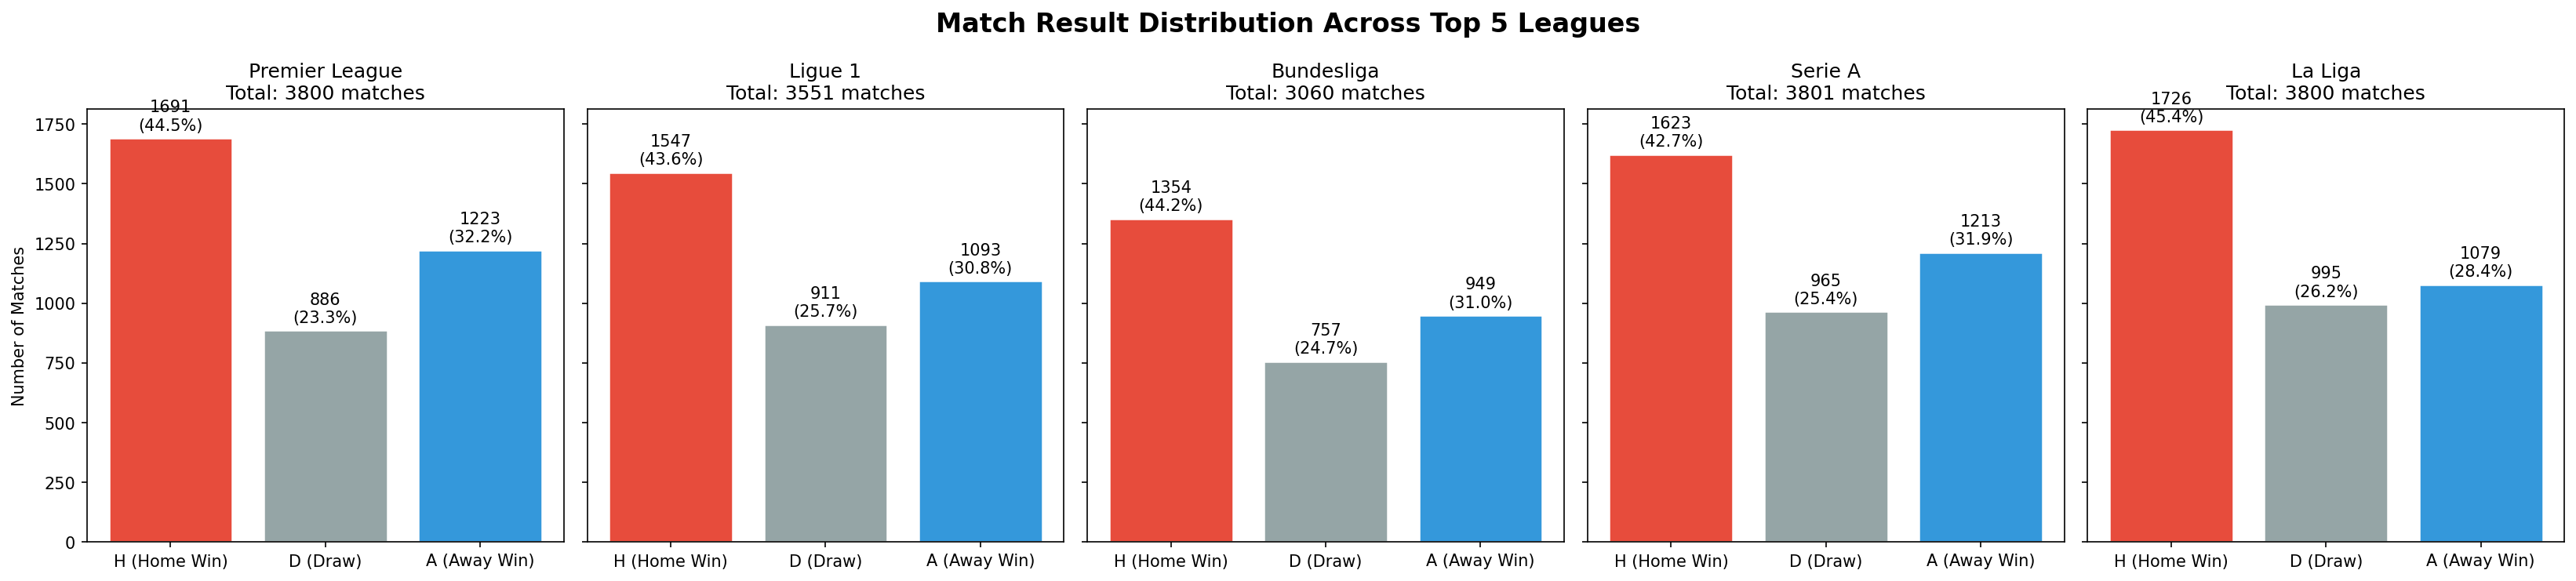
\includegraphics[width=0.95\textwidth]{../outputs/league_data_analysis/1_league_result_distribution.png}
\caption{Outcome distribution per league across seasons 2015/16--2024/25.
Home wins dominate every league, with draws as the minority class.}
\label{fig:result-dist}
\end{figure}

A side-by-side comparison of the per-class shares
(Figure~\ref{fig:result-comparison}) confirms that home advantage is
the most stable pre-match prior across leagues; the draw share is also
remarkably stable at $24$--$26\%$, while the away-win share absorbs
most of the league-to-league variation.

\begin{figure}[h]
\centering
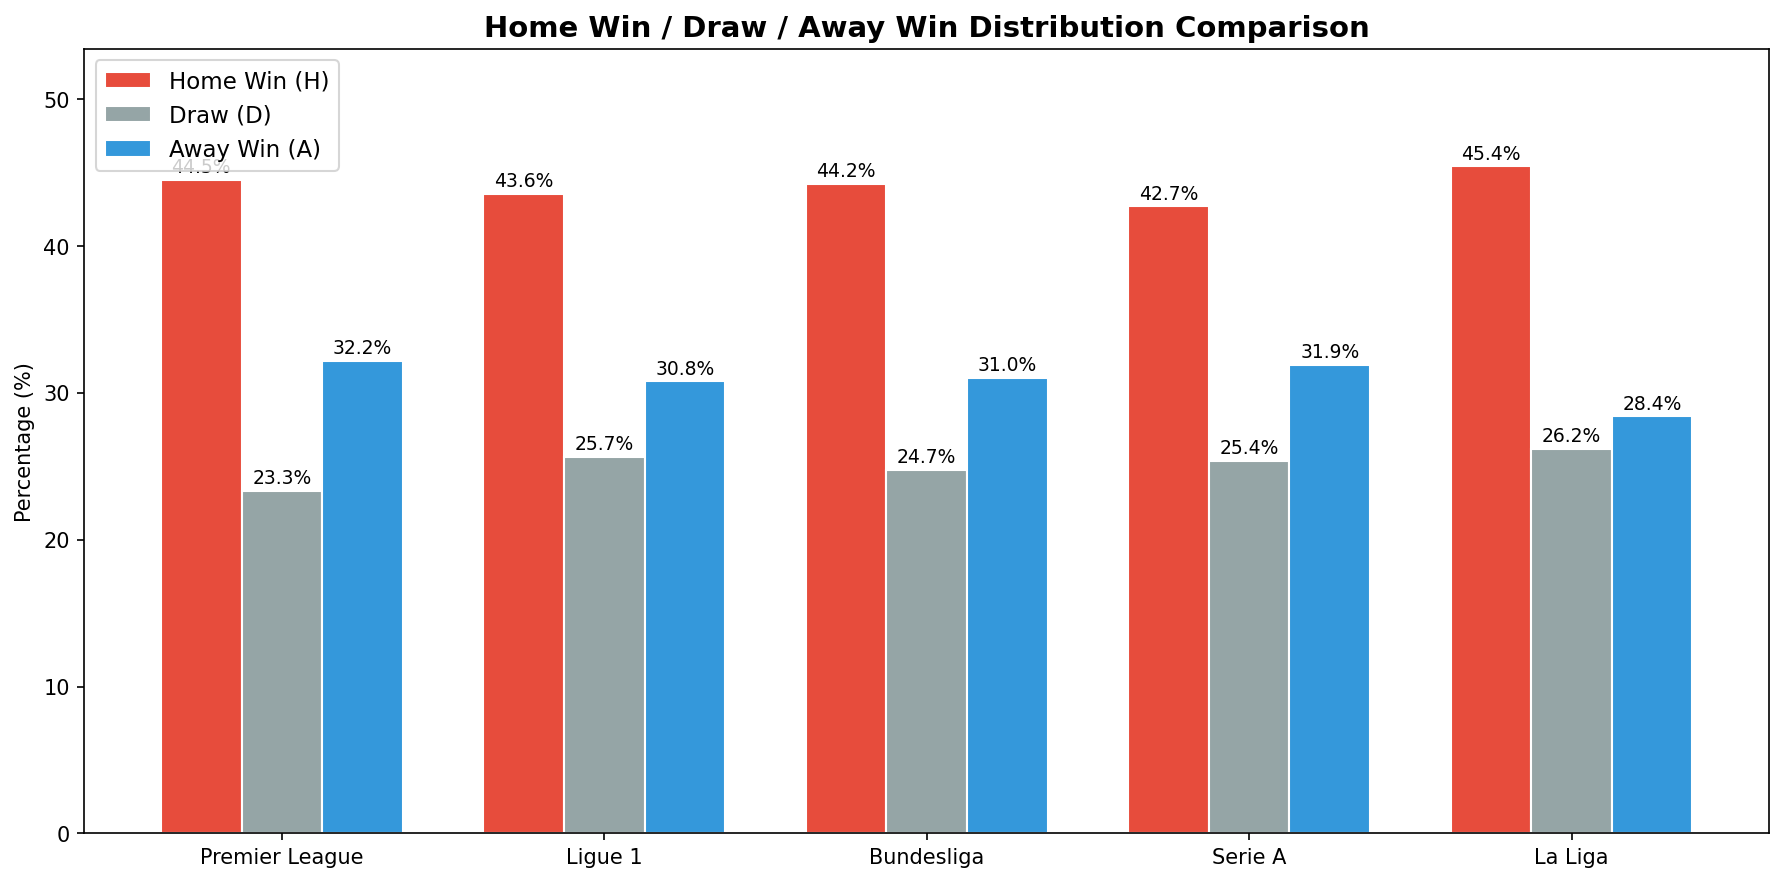
\includegraphics[width=0.95\textwidth]{../outputs/league_data_analysis/2_league_result_comparison.png}
\caption{Per-class share by league (H/D/A). Home advantage is the
dominant pre-match prior; the draw rate is stable at $\sim$$0.24$
across all five leagues.}
\label{fig:result-comparison}
\end{figure}

\paragraph{Team-level home / away / draw breakdown.}
Figures~\ref{fig:team-eng}--\ref{fig:team-fra} (released in
\texttt{outputs/league\_data\_analysis/3\_*\_team\_home\_away\_draw.png})
break the per-league outcome distribution down to the team level.
Three patterns emerge that are relevant to the model. First, the top
clubs in every league concentrate the home-win mass: Manchester~City,
Liverpool, Real~Madrid, Barcelona, Bayern, Juventus, Inter, and PSG
each contribute substantially more home wins than the league average,
which means a learner that uses team-rating features (Elo, PPG,
historical win-rate) will inherit useful structure even before
considering odds. Second, mid-table sides cluster around the league
mean, so the per-team variance among that group is dominated by
short-run form rather than a stable rating, and the form / momentum
features in Stage~4 (Section~\ref{subsec:form}) are designed for
exactly that regime. Third, draw counts are the flattest curve across
clubs, reinforcing that draws are intrinsically harder to attribute
to a stable team-level prior than home or away wins.

\paragraph{Odds distribution and market consensus.}
The bookmaker market provides the single most informative pre-match
covariate, and Figures~\ref{fig:odds-pooled}--\ref{fig:odds-by-result}
characterise it. The pooled distribution of decimal closing odds
(Figure~\ref{fig:odds-pooled}) is heavily right-skewed for the away
column and approximately log-normal for the home column, with the
draw column tightly concentrated in the $3.0$--$3.6$ band as expected
from the bookmaker convention of pricing draws around the $1/3$
implied-probability margin. Per-league odds histograms
(Figures~\ref{fig:odds-eng}--\ref{fig:odds-fra}, released as
\texttt{4\_*\_odds\_distribution.png}) confirm that this shape is
stable across leagues, with the Bundesliga showing slightly fatter
tails on the away column---consistent with its more competitive
balance and the larger feature-importance scores observed for
\texttt{odds\_ft\_*} in the German feature-ranking
(Table~\ref{tab:fi-ger}).

\begin{figure}[h]
\centering
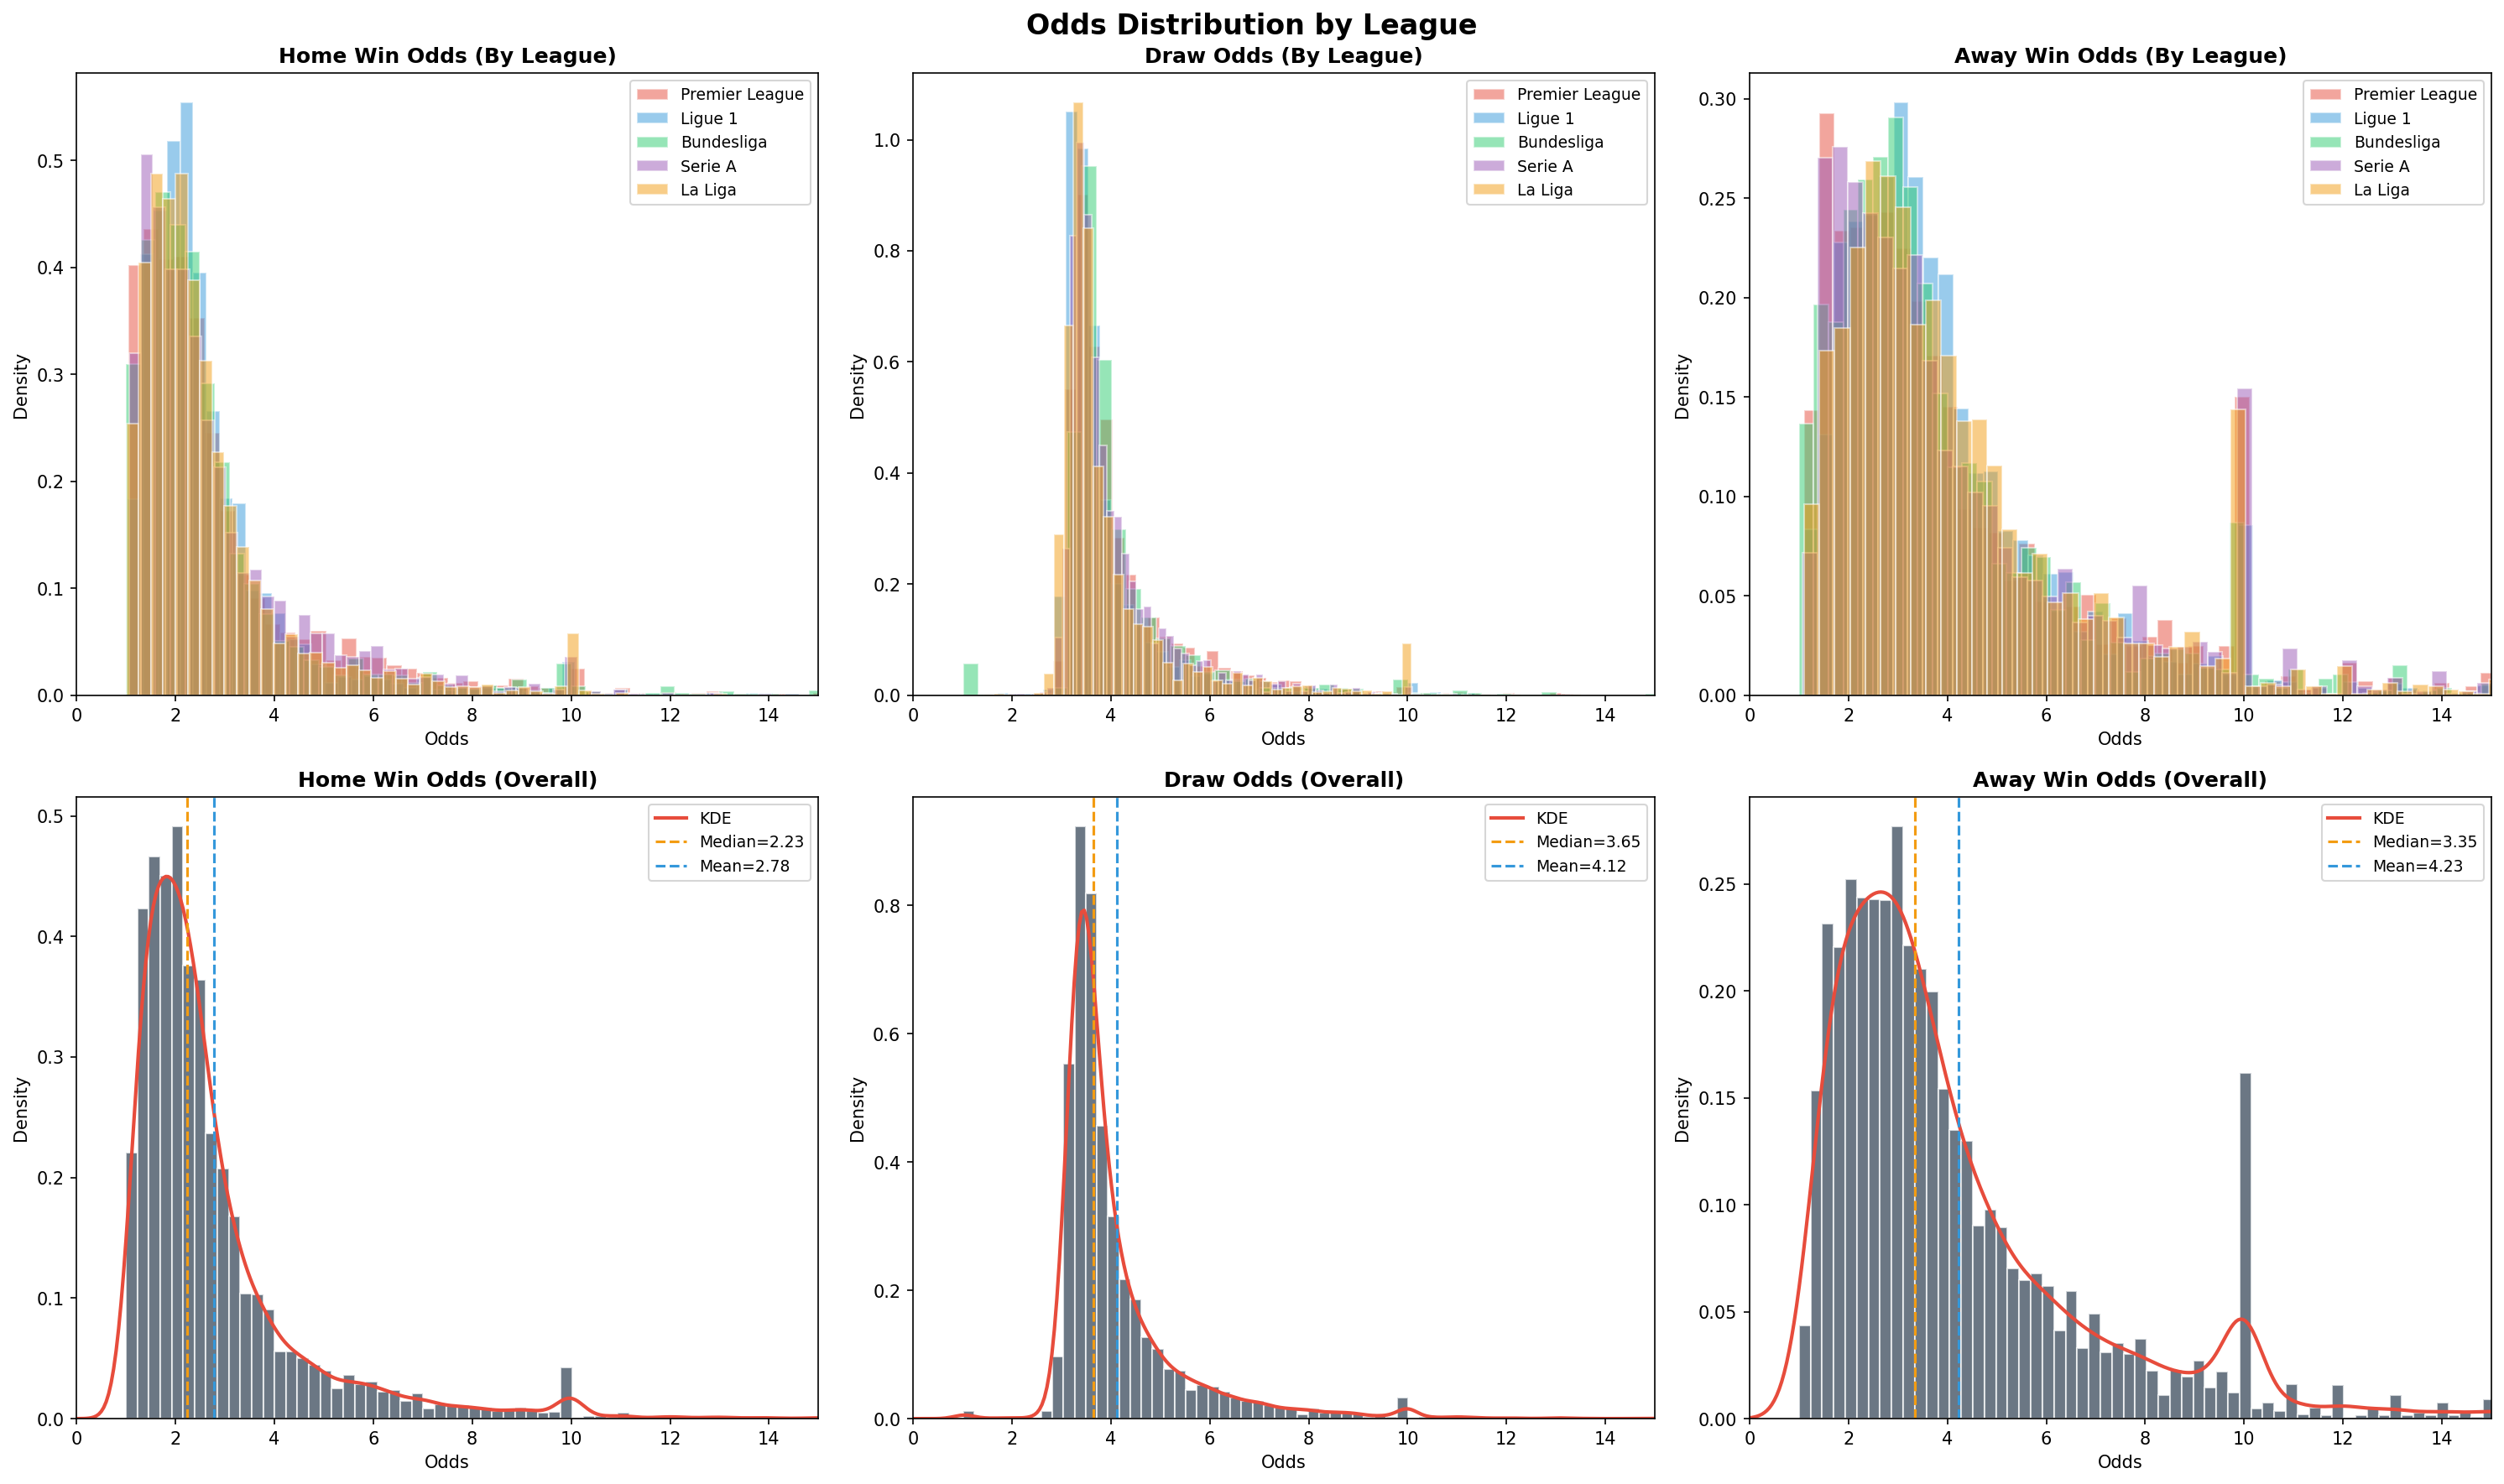
\includegraphics[width=0.95\textwidth]{../outputs/league_data_analysis/4_odds_distribution.png}
\caption{Pooled distribution of closing odds (1X2 market) across the
five leagues. The draw column is tightly concentrated; the away
column is the most dispersed.}
\label{fig:odds-pooled}
\end{figure}

When the same odds are stratified by realised outcome
(Figure~\ref{fig:odds-by-result}), the market emerges as a
near-monotonic predictor: matches that ended in home wins are
heavily weighted toward low \texttt{odds\_ft\_home\_team\_win} (the
favourites won), away wins concentrate at low
\texttt{odds\_ft\_away\_team\_win}, and draws sit close to the
overall median in every column. This confirms market efficiency at
the population level and explains why the odds family dominates the
Random-Forest importance ranking
(Section~\ref{subsec:fi-analysis}, Table~\ref{tab:fi-universal}):
under perfect market efficiency the implied-probability vector
would be the Bayes-optimal pre-match feature, and our results show
the deviation from that limit is small.

\begin{figure}[h]
\centering
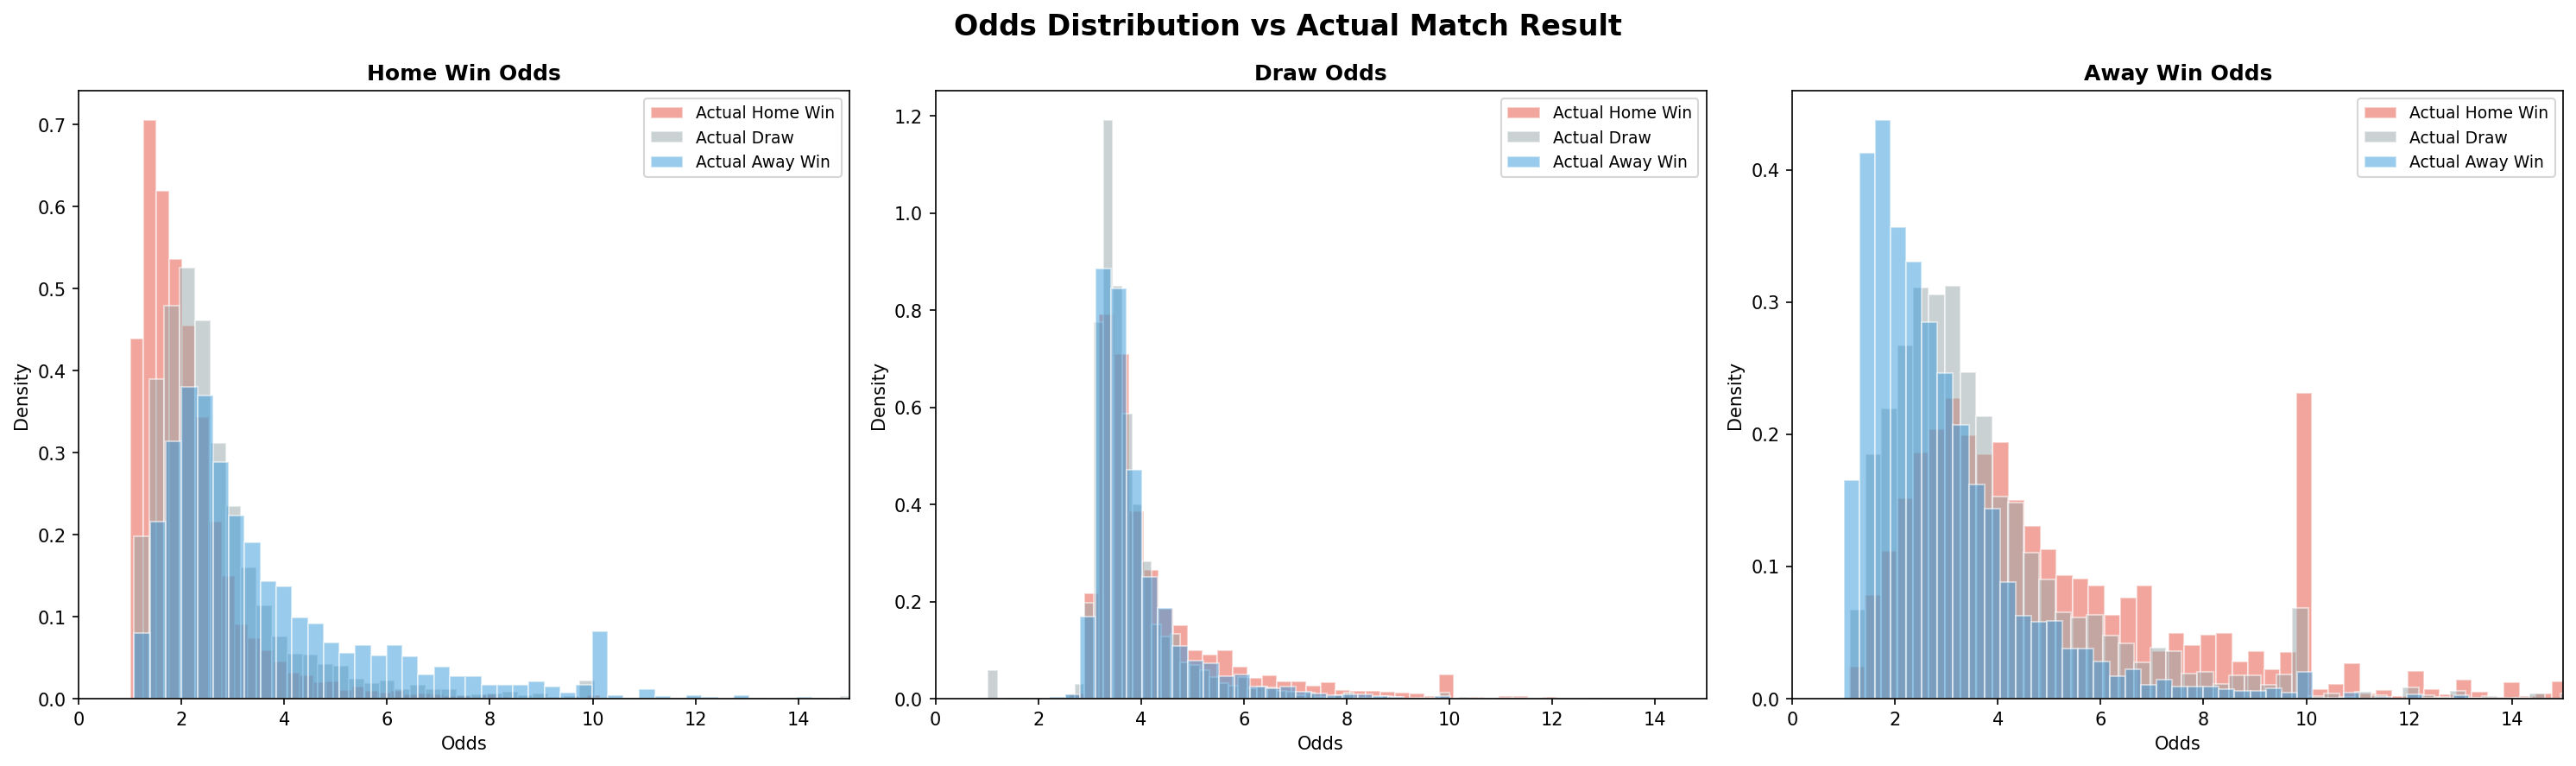
\includegraphics[width=0.95\textwidth]{../outputs/league_data_analysis/5_odds_by_result.png}
\caption{Closing-odds distribution stratified by realised outcome
(H/D/A). The market is near-monotonic: low \texttt{odds\_ft\_home\_team\_win}
correlates strongly with home wins; analogous patterns hold for the
away column.}
\label{fig:odds-by-result}
\end{figure}

\paragraph{Implications for modelling.}
Three modelling decisions follow directly from the distributions
above. (i)~The draw class must be reported separately because no
single feature carries a strong draw signal in any league, and a
weighted-average metric would mask draw collapse; this motivates the
F1-macro headline metric. (ii)~Market odds and Elo together account
for the bulk of the predictable home/away variation, so non-odds
features must clear a meaningful incremental bar to justify
inclusion---a hypothesis tested directly by the feature-importance
analysis in Section~\ref{subsec:fi-analysis}. (iii)~Per-league
imbalance and home-advantage are similar enough that a single
pipeline trained per league is appropriate; cross-league transfer is
left to future work.

%% =====================================================================

%% 8. RESULTS
%% =====================================================================
\section{Results}\label{sec:results}

\subsection{Pre-match prediction}\label{subsec:res-pre}

Tables~\ref{tab:pre-eng}--\ref{tab:pre-fra} report pre-match
performance for the five leagues separately on the held-out
$2023/24$ test season, using the model space defined in
Section~\ref{sec:method} and the protocol described in
Section~\ref{sec:setup}. Table~\ref{tab:pre-perclass} complements
the per-league summaries with the pooled per-class precision,
recall and F1 breakdown over the three outcome labels, following the
format of prior work.

\begin{table}[h]
\caption{Pre-match results for England (Premier League) on the held-out
$2023/24$ test season.}\label{tab:pre-eng}
\begin{tabular}{@{}lccccc@{}}
\toprule
Model               & Accuracy & F1-macro & Log-loss & AUC-macro & Draw F1 \\
\midrule
Logistic Regression & TBD & TBD & TBD & TBD & TBD \\
Gaussian NB         & TBD & TBD & TBD & TBD & TBD \\
Linear SVM (cal.)   & TBD & TBD & TBD & TBD & TBD \\
Random Forest       & TBD & TBD & TBD & TBD & TBD \\
XGBoost             & TBD & TBD & TBD & TBD & TBD \\
Vanilla RNN         & TBD & TBD & TBD & TBD & TBD \\
Feed-forward NN     & TBD & TBD & TBD & TBD & TBD \\
\midrule
Voting (soft)       & TBD & TBD & TBD & TBD & TBD \\
Stacking (LR meta)  & TBD & TBD & TBD & TBD & TBD \\
\botrule
\end{tabular}
\end{table}

\begin{table}[h]
\caption{Pre-match results for Spain (La Liga) on the held-out
$2023/24$ test season.}\label{tab:pre-esp}
\begin{tabular}{@{}lccccc@{}}
\toprule
Model               & Accuracy & F1-macro & Log-loss & AUC-macro & Draw F1 \\
\midrule
Logistic Regression & TBD & TBD & TBD & TBD & TBD \\
Gaussian NB         & TBD & TBD & TBD & TBD & TBD \\
Linear SVM (cal.)   & TBD & TBD & TBD & TBD & TBD \\
Random Forest       & TBD & TBD & TBD & TBD & TBD \\
XGBoost             & TBD & TBD & TBD & TBD & TBD \\
Vanilla RNN         & TBD & TBD & TBD & TBD & TBD \\
Feed-forward NN     & TBD & TBD & TBD & TBD & TBD \\
\midrule
Voting (soft)       & TBD & TBD & TBD & TBD & TBD \\
Stacking (LR meta)  & TBD & TBD & TBD & TBD & TBD \\
\botrule
\end{tabular}
\end{table}

\begin{table}[h]
\caption{Pre-match results for Germany (Bundesliga) on the held-out
$2023/24$ test season.}\label{tab:pre-ger}
\begin{tabular}{@{}lccccc@{}}
\toprule
Model               & Accuracy & F1-macro & Log-loss & AUC-macro & Draw F1 \\
\midrule
Logistic Regression & TBD & TBD & TBD & TBD & TBD \\
Gaussian NB         & TBD & TBD & TBD & TBD & TBD \\
Linear SVM (cal.)   & TBD & TBD & TBD & TBD & TBD \\
Random Forest       & TBD & TBD & TBD & TBD & TBD \\
XGBoost             & TBD & TBD & TBD & TBD & TBD \\
Vanilla RNN         & TBD & TBD & TBD & TBD & TBD \\
Feed-forward NN     & TBD & TBD & TBD & TBD & TBD \\
\midrule
Voting (soft)       & TBD & TBD & TBD & TBD & TBD \\
Stacking (LR meta)  & TBD & TBD & TBD & TBD & TBD \\
\botrule
\end{tabular}
\end{table}

\begin{table}[h]
\caption{Pre-match results for Italy (Serie A) on the held-out
$2023/24$ test season.}\label{tab:pre-ita}
\begin{tabular}{@{}lccccc@{}}
\toprule
Model               & Accuracy & F1-macro & Log-loss & AUC-macro & Draw F1 \\
\midrule
Logistic Regression & TBD & TBD & TBD & TBD & TBD \\
Gaussian NB         & TBD & TBD & TBD & TBD & TBD \\
Linear SVM (cal.)   & TBD & TBD & TBD & TBD & TBD \\
Random Forest       & TBD & TBD & TBD & TBD & TBD \\
XGBoost             & TBD & TBD & TBD & TBD & TBD \\
Vanilla RNN         & TBD & TBD & TBD & TBD & TBD \\
Feed-forward NN     & TBD & TBD & TBD & TBD & TBD \\
\midrule
Voting (soft)       & TBD & TBD & TBD & TBD & TBD \\
Stacking (LR meta)  & TBD & TBD & TBD & TBD & TBD \\
\botrule
\end{tabular}
\end{table}

\begin{table}[h]
\caption{Pre-match results for France (Ligue 1) on the held-out
$2023/24$ test season.}\label{tab:pre-fra}
\begin{tabular}{@{}lccccc@{}}
\toprule
Model               & Accuracy & F1-macro & Log-loss & AUC-macro & Draw F1 \\
\midrule
Logistic Regression & TBD & TBD & TBD & TBD & TBD \\
Gaussian NB         & TBD & TBD & TBD & TBD & TBD \\
Linear SVM (cal.)   & TBD & TBD & TBD & TBD & TBD \\
Random Forest       & TBD & TBD & TBD & TBD & TBD \\
XGBoost             & TBD & TBD & TBD & TBD & TBD \\
Vanilla RNN         & TBD & TBD & TBD & TBD & TBD \\
Feed-forward NN     & TBD & TBD & TBD & TBD & TBD \\
\midrule
Voting (soft)       & TBD & TBD & TBD & TBD & TBD \\
Stacking (LR meta)  & TBD & TBD & TBD & TBD & TBD \\
\botrule
\end{tabular}
\end{table}

\begin{table}[h]
\caption{Per-class classification metrics (Precision, Recall, F1) on
the pre-match task, pooled across the five leagues on the $2023/24$
test season.}\label{tab:pre-perclass}
\footnotesize
\begin{tabular*}{\textwidth}{@{\extracolsep\fill}llccc@{}}
\toprule
Model & Class & Precision & Recall & F1 \\
\midrule
\multirow{3}{*}{Logistic Regression} & Home (0) & TBD & TBD & TBD \\
                                     & Draw (1) & TBD & TBD & TBD \\
                                     & Away (2) & TBD & TBD & TBD \\
\midrule
\multirow{3}{*}{Gaussian NB}         & Home (0) & TBD & TBD & TBD \\
                                     & Draw (1) & TBD & TBD & TBD \\
                                     & Away (2) & TBD & TBD & TBD \\
\midrule
\multirow{3}{*}{Linear SVM (cal.)}   & Home (0) & TBD & TBD & TBD \\
                                     & Draw (1) & TBD & TBD & TBD \\
                                     & Away (2) & TBD & TBD & TBD \\
\midrule
\multirow{3}{*}{Random Forest}       & Home (0) & TBD & TBD & TBD \\
                                     & Draw (1) & TBD & TBD & TBD \\
                                     & Away (2) & TBD & TBD & TBD \\
\midrule
\multirow{3}{*}{XGBoost}             & Home (0) & TBD & TBD & TBD \\
                                     & Draw (1) & TBD & TBD & TBD \\
                                     & Away (2) & TBD & TBD & TBD \\
\midrule
\multirow{3}{*}{Vanilla RNN}         & Home (0) & TBD & TBD & TBD \\
                                     & Draw (1) & TBD & TBD & TBD \\
                                     & Away (2) & TBD & TBD & TBD \\
\midrule
\multirow{3}{*}{Feed-forward NN}     & Home (0) & TBD & TBD & TBD \\
                                     & Draw (1) & TBD & TBD & TBD \\
                                     & Away (2) & TBD & TBD & TBD \\
\midrule
\multirow{3}{*}{Voting (soft)}       & Home (0) & TBD & TBD & TBD \\
                                     & Draw (1) & TBD & TBD & TBD \\
                                     & Away (2) & TBD & TBD & TBD \\
\midrule
\multirow{3}{*}{Stacking (LR meta)}  & Home (0) & TBD & TBD & TBD \\
                                     & Draw (1) & TBD & TBD & TBD \\
                                     & Away (2) & TBD & TBD & TBD \\
\botrule
\end{tabular*}
\end{table}

\paragraph{Hyper-parameter configuration.}
\emph{[Placeholder --- to describe, per model, the search strategy
(grid vs.\ random), the cross-validation protocol, the scoring
function, and the best configuration selected for each league.]}

\paragraph{Analysis.}
\emph{[Placeholder --- reserved for discussion of model ranking,
draw-class performance, and per-league differences once the full
set of runs is complete.]}

\subsection{Half-time prediction}\label{subsec:res-ht}

Tables~\ref{tab:ht-eng}--\ref{tab:ht-fra} report half-time
performance for the five leagues separately under the same protocol,
and Table~\ref{tab:ht-perclass} reports the pooled per-class
breakdown. Incorporating the seven half-time columns is expected to
yield a substantial uplift over pre-match prediction across every
learner.

\begin{table}[h]
\caption{Half-time results for England (Premier League) on the
held-out $2023/24$ test season.}\label{tab:ht-eng}
\begin{tabular}{@{}lccccc@{}}
\toprule
Model               & Accuracy & F1-macro & Log-loss & AUC-macro & Draw F1 \\
\midrule
Logistic Regression & TBD & TBD & TBD & TBD & TBD \\
Gaussian NB         & TBD & TBD & TBD & TBD & TBD \\
Linear SVM (cal.)   & TBD & TBD & TBD & TBD & TBD \\
Random Forest       & TBD & TBD & TBD & TBD & TBD \\
XGBoost             & TBD & TBD & TBD & TBD & TBD \\
Vanilla RNN         & TBD & TBD & TBD & TBD & TBD \\
Feed-forward NN     & TBD & TBD & TBD & TBD & TBD \\
\midrule
Voting (soft)       & TBD & TBD & TBD & TBD & TBD \\
Stacking (LR meta)  & TBD & TBD & TBD & TBD & TBD \\
\botrule
\end{tabular}
\end{table}

\begin{table}[h]
\caption{Half-time results for Spain (La Liga) on the held-out
$2023/24$ test season.}\label{tab:ht-esp}
\begin{tabular}{@{}lccccc@{}}
\toprule
Model               & Accuracy & F1-macro & Log-loss & AUC-macro & Draw F1 \\
\midrule
Logistic Regression & TBD & TBD & TBD & TBD & TBD \\
Gaussian NB         & TBD & TBD & TBD & TBD & TBD \\
Linear SVM (cal.)   & TBD & TBD & TBD & TBD & TBD \\
Random Forest       & TBD & TBD & TBD & TBD & TBD \\
XGBoost             & TBD & TBD & TBD & TBD & TBD \\
Vanilla RNN         & TBD & TBD & TBD & TBD & TBD \\
Feed-forward NN     & TBD & TBD & TBD & TBD & TBD \\
\midrule
Voting (soft)       & TBD & TBD & TBD & TBD & TBD \\
Stacking (LR meta)  & TBD & TBD & TBD & TBD & TBD \\
\botrule
\end{tabular}
\end{table}

\begin{table}[h]
\caption{Half-time results for Germany (Bundesliga) on the held-out
$2023/24$ test season.}\label{tab:ht-ger}
\begin{tabular}{@{}lccccc@{}}
\toprule
Model               & Accuracy & F1-macro & Log-loss & AUC-macro & Draw F1 \\
\midrule
Logistic Regression & TBD & TBD & TBD & TBD & TBD \\
Gaussian NB         & TBD & TBD & TBD & TBD & TBD \\
Linear SVM (cal.)   & TBD & TBD & TBD & TBD & TBD \\
Random Forest       & TBD & TBD & TBD & TBD & TBD \\
XGBoost             & TBD & TBD & TBD & TBD & TBD \\
Vanilla RNN         & TBD & TBD & TBD & TBD & TBD \\
Feed-forward NN     & TBD & TBD & TBD & TBD & TBD \\
\midrule
Voting (soft)       & TBD & TBD & TBD & TBD & TBD \\
Stacking (LR meta)  & TBD & TBD & TBD & TBD & TBD \\
\botrule
\end{tabular}
\end{table}

\begin{table}[h]
\caption{Half-time results for Italy (Serie A) on the held-out
$2023/24$ test season.}\label{tab:ht-ita}
\begin{tabular}{@{}lccccc@{}}
\toprule
Model               & Accuracy & F1-macro & Log-loss & AUC-macro & Draw F1 \\
\midrule
Logistic Regression & TBD & TBD & TBD & TBD & TBD \\
Gaussian NB         & TBD & TBD & TBD & TBD & TBD \\
Linear SVM (cal.)   & TBD & TBD & TBD & TBD & TBD \\
Random Forest       & TBD & TBD & TBD & TBD & TBD \\
XGBoost             & TBD & TBD & TBD & TBD & TBD \\
Vanilla RNN         & TBD & TBD & TBD & TBD & TBD \\
Feed-forward NN     & TBD & TBD & TBD & TBD & TBD \\
\midrule
Voting (soft)       & TBD & TBD & TBD & TBD & TBD \\
Stacking (LR meta)  & TBD & TBD & TBD & TBD & TBD \\
\botrule
\end{tabular}
\end{table}

\begin{table}[h]
\caption{Half-time results for France (Ligue 1) on the held-out
$2023/24$ test season.}\label{tab:ht-fra}
\begin{tabular}{@{}lccccc@{}}
\toprule
Model               & Accuracy & F1-macro & Log-loss & AUC-macro & Draw F1 \\
\midrule
Logistic Regression & TBD & TBD & TBD & TBD & TBD \\
Gaussian NB         & TBD & TBD & TBD & TBD & TBD \\
Linear SVM (cal.)   & TBD & TBD & TBD & TBD & TBD \\
Random Forest       & TBD & TBD & TBD & TBD & TBD \\
XGBoost             & TBD & TBD & TBD & TBD & TBD \\
Vanilla RNN         & TBD & TBD & TBD & TBD & TBD \\
Feed-forward NN     & TBD & TBD & TBD & TBD & TBD \\
\midrule
Voting (soft)       & TBD & TBD & TBD & TBD & TBD \\
Stacking (LR meta)  & TBD & TBD & TBD & TBD & TBD \\
\botrule
\end{tabular}
\end{table}

\begin{table}[h]
\caption{Per-class classification metrics (Precision, Recall, F1) on
the half-time task, pooled across the five leagues on the $2023/24$
test season.}\label{tab:ht-perclass}
\footnotesize
\begin{tabular*}{\textwidth}{@{\extracolsep\fill}llccc@{}}
\toprule
Model & Class & Precision & Recall & F1 \\
\midrule
\multirow{3}{*}{Logistic Regression} & Home (0) & TBD & TBD & TBD \\
                                     & Draw (1) & TBD & TBD & TBD \\
                                     & Away (2) & TBD & TBD & TBD \\
\midrule
\multirow{3}{*}{Gaussian NB}         & Home (0) & TBD & TBD & TBD \\
                                     & Draw (1) & TBD & TBD & TBD \\
                                     & Away (2) & TBD & TBD & TBD \\
\midrule
\multirow{3}{*}{Linear SVM (cal.)}   & Home (0) & TBD & TBD & TBD \\
                                     & Draw (1) & TBD & TBD & TBD \\
                                     & Away (2) & TBD & TBD & TBD \\
\midrule
\multirow{3}{*}{Random Forest}       & Home (0) & TBD & TBD & TBD \\
                                     & Draw (1) & TBD & TBD & TBD \\
                                     & Away (2) & TBD & TBD & TBD \\
\midrule
\multirow{3}{*}{XGBoost}             & Home (0) & TBD & TBD & TBD \\
                                     & Draw (1) & TBD & TBD & TBD \\
                                     & Away (2) & TBD & TBD & TBD \\
\midrule
\multirow{3}{*}{Vanilla RNN}         & Home (0) & TBD & TBD & TBD \\
                                     & Draw (1) & TBD & TBD & TBD \\
                                     & Away (2) & TBD & TBD & TBD \\
\midrule
\multirow{3}{*}{Feed-forward NN}     & Home (0) & TBD & TBD & TBD \\
                                     & Draw (1) & TBD & TBD & TBD \\
                                     & Away (2) & TBD & TBD & TBD \\
\midrule
\multirow{3}{*}{Voting (soft)}       & Home (0) & TBD & TBD & TBD \\
                                     & Draw (1) & TBD & TBD & TBD \\
                                     & Away (2) & TBD & TBD & TBD \\
\midrule
\multirow{3}{*}{Stacking (LR meta)}  & Home (0) & TBD & TBD & TBD \\
                                     & Draw (1) & TBD & TBD & TBD \\
                                     & Away (2) & TBD & TBD & TBD \\
\botrule
\end{tabular*}
\end{table}

\paragraph{Hyper-parameter configuration.}
\emph{[Placeholder --- as in the pre-match task, to be expanded with
the search strategy, cross-validation protocol, scoring function,
and selected configurations for the half-time task.]}

\paragraph{Analysis.}
\emph{[Placeholder --- reserved for future expansion.]}

\subsection{Real-time momentum comparison}\label{subsec:res-mom}

Table~\ref{tab:mom-overview} compares every learner on the
$2015/16$ season pooled across the five leagues, with and without
the real-time momentum feature block, for both the pre-match and
half-time tasks.

\begin{table}[h]
\caption{Pre-match and half-time performance on the $2015/16$
season pooled across the five leagues, with and without the
real-time momentum feature block. Each cell is reported as
Accuracy\,/\,F1-macro.}\label{tab:mom-overview}
\footnotesize
\begin{tabular*}{\textwidth}{@{\extracolsep\fill}l cc cc@{}}
\toprule
 & \multicolumn{2}{c}{\textbf{Pre-match}} & \multicolumn{2}{c}{\textbf{Half-time}} \\
\cmidrule(r){2-3}\cmidrule(l){4-5}
Model               & Without mom. & With mom. & Without mom. & With mom. \\
\midrule
Logistic Regression & TBD\,/\,TBD & TBD\,/\,TBD & TBD\,/\,TBD & TBD\,/\,TBD \\
Gaussian NB         & TBD\,/\,TBD & TBD\,/\,TBD & TBD\,/\,TBD & TBD\,/\,TBD \\
Linear SVM (cal.)   & TBD\,/\,TBD & TBD\,/\,TBD & TBD\,/\,TBD & TBD\,/\,TBD \\
Random Forest       & TBD\,/\,TBD & TBD\,/\,TBD & TBD\,/\,TBD & TBD\,/\,TBD \\
XGBoost             & TBD\,/\,TBD & TBD\,/\,TBD & TBD\,/\,TBD & TBD\,/\,TBD \\
Vanilla RNN         & TBD\,/\,TBD & TBD\,/\,TBD & TBD\,/\,TBD & TBD\,/\,TBD \\
Feed-forward NN     & TBD\,/\,TBD & TBD\,/\,TBD & TBD\,/\,TBD & TBD\,/\,TBD \\
\midrule
Voting (soft)       & TBD\,/\,TBD & TBD\,/\,TBD & TBD\,/\,TBD & TBD\,/\,TBD \\
Stacking (LR meta)  & TBD\,/\,TBD & TBD\,/\,TBD & TBD\,/\,TBD & TBD\,/\,TBD \\
\botrule
\end{tabular*}
\end{table}

\paragraph{Hyper-parameter configuration.}
\emph{[Placeholder --- describe the tuning protocol used for the
momentum ablation and whether it mirrors the main runs, including
cross-validation setup.]}

\paragraph{Analysis.}
\emph{[Placeholder --- reserved for future expansion.]}

\subsection{Comparison within the five leagues}\label{subsec:res-cross}

\emph{[Placeholder --- reserved for future expansion; will
cross-compare the best model's per-league performance
(Tables~\ref{tab:pre-eng}--\ref{tab:pre-fra} and
\ref{tab:ht-eng}--\ref{tab:ht-fra}) to identify systematic
differences in difficulty and in the set of informative features.]}

%% =====================================================================
%% 9. DISCUSSION
%% =====================================================================
\section{Discussion}\label{sec:discussion}
\emph{[Placeholder --- content to be added in a future revision.]}



%% =====================================================================
%% 10. CONCLUSION
%% =====================================================================
\section{Conclusion}\label{sec:conclusion}

\emph{[Placeholder --- content to be added in a future revision.]}

%% =====================================================================
%% BACKMATTER
%% =====================================================================
\backmatter

\bmhead{Supplementary information}
The full source code, configuration files, trained model artifacts, and
per-league reports are released at \url{https://github.com/Corey30/SoccerPre}.

\bmhead{Acknowledgements}
The authors thank \dots{} for helpful discussions and acknowledge
support from \dots{}.

\section*{Declarations}
\begin{itemize}
  \item \textbf{Funding}: not applicable.
  \item \textbf{Conflict of interest}: the authors declare no competing
        interests.
  \item \textbf{Ethics approval and consent to participate}: not
        applicable. The study uses publicly available match-level
        statistics; no human subjects are involved.
  \item \textbf{Data availability}: derived datasets and pipeline
        scripts are released alongside the source code.
  \item \textbf{Code availability}: as above.
  \item \textbf{Author contribution}: \dots{}.
\end{itemize}

\begin{appendices}

\section{Hyper-parameter configurations}\label{secA1}

The exact configurations used for the reported results are listed in
Table~\ref{tab:hparams}. Values reflect the production settings in the
released pipeline.

\begin{table}[h]
\caption{Default hyper-parameters for each base learner.}\label{tab:hparams}
\begin{tabular*}{\textwidth}{@{\extracolsep\fill}ll@{}}
\toprule
Model               & Settings \\
\midrule
Logistic Regression & $C\!=\!0.5$, L2, lbfgs, max\_iter $\!=\!3000$, custom class weight $\{H{:}1.0,D{:}2.8,A{:}1.0\}$ \\
Gaussian NB         & var\_smoothing $\!=\!10^{-8}$ \\
Linear SVM          & $C\!=\!2.0$, max\_iter $\!=\!2\!\times\!10^4$, class weight $\{H{:}1.0,D{:}5.0,A{:}1.0\}$, calibrated \\
Random Forest       & 180 trees, max\_depth 8, min\_samples\_leaf 2, max\_features sqrt, custom class weight \\
XGBoost             & 150 trees, max\_depth 5, $\eta\!=\!0.06$, subsample 0.75, colsample 0.75, $L_2\!=\!1.5$, $L_1\!=\!0.2$, $\gamma\!=\!0.06$ \\
Feed-forward NN     & layers $(100,50)$, ReLU, Adam, lr $\!=\!6\!\times\!10^{-4}$, $\alpha\!=\!0.5$, batch 64, early stopping \\
\botrule
\end{tabular*}
\end{table}

\section{Feature catalogue}\label{secA2}

The released pipeline produces approximately $150$ numeric pre-match
features and $7$ additional half-time features. The complete list,
together with type-aware imputation rules, is provided in the project
repository as \texttt{src/config/config.py} and
\texttt{src/features/prematch\_features.py}.

\end{appendices}

%% =====================================================================
%% BIBLIOGRAPHY (replace with actual entries from your literature review)
%% =====================================================================
\begin{thebibliography}{99}
\bibitem{bib1} Author A., Author B.: Title. Journal \textbf{1}(1), 1--20 (2020).
\bibitem{bib2} Author C.: Title. Journal \textbf{2}(2), 1--20 (2021).
\bibitem{bib3} Maher, M.J.: Modelling association football scores. Statistica Neerlandica \textbf{36}, 109--118 (1982).
\bibitem{bib4} Dixon, M.J., Coles, S.G.: Modelling association football scores and inefficiencies in the football betting market. Applied Statistics \textbf{46}(2), 265--280 (1997).
\bibitem{bib5} Author E.: Title. Journal \textbf{5}(5), 1--20 (2019).
\bibitem{bib6} Author F.: Title. Journal \textbf{6}(6), 1--20 (2022).
\bibitem{bib7} Author G.: Title. Journal \textbf{7}(7), 1--20 (2023).
\bibitem{bib8} Author H.: Title. Journal \textbf{8}(8), 1--20 (2023).
\bibitem{bib9} Author I.: Title. Journal \textbf{9}(9), 1--20 (2024).
\bibitem{bib10} Author J.: Title. Journal \textbf{10}(10), 1--20 (2024).
\bibitem{bib11} Reference paper of professor (placeholder).

\end{thebibliography}

\end{document}